%\documentclass[smaller, handout]{beamer}
\def\bmode{0} % Mode 0 for presentation, mode 1 for a handout with notes, mode 2 fo% r handout without notes
\if 0\bmode
\documentclass[smaller]{beamer}
\else \if 1\bmode
\immediate\write18{pdflatex -jobname=\jobname-Handout-Notes\space\jobname}
\documentclass[smaller,handout]{beamer}
\usepackage{handoutWithNotes}
\pgfpagesuselayout{2 on 1 with notes}[letterpaper, landscape, border shrink=4mm]
\else \if 2\bmode
\immediate\write18{pdflatex -jobname=\jobname-Handout\space\jobname}
\documentclass[smaller,handout]{beamer}
\fi
\fi
\fi

%\setbeamertemplate{section in head/foot}{}
%\setbeamertemplate{section in head/foot shaded}{\textcolor{white}{\insertsectionhead}}
%%%%%%%%%%%%%%%%%%%%%%%%%%%%%%%%%%%%%%%%%%%%%%%%%%%%%%%%%%%%%%%%%%%%%%%%%%%%%%%%%%%%%%%%%%%%%
\newcommand{\coursetitle}{CEE 616: Probabilistic Machine Learning}
\newcommand{\longlecturetitle}{M3 Deep Neural Networks:\\ Lecture 3D: Neural Networks for Sequences}
\newcommand{\shortlecturetitle}{3D: NNs for Sequences}
\newcommand{\instructor}{Jimi Oke}
\newcommand{\lecturedate}{Tue, Oct 28, 2025}
%%%%%%%%%%%%%%%%%%%%%%%%%%%%%%%%%%%%%%%%%%%%%%%%%%%%%%%%%%%%%%%%%%%%%%%%%%%%%%%%%%%%%%%%%%%%%

 
 
% \usepackage[T1]{fontenc} 
% \usepackage{lmodern} 
%\usepackage{etex}
 %\newcommand{\num}{6{} }

% \usetheme[
%   outer/progressbar=foot,
%   outer/numbering=fraction,
%   block=fill,
%   inner/subsectionpage=progressbar
% ]{metropolis}
\usetheme{Madrid}
\useoutertheme[subsection=false]{miniframes} % Alternatively: miniframes, infolines, split
\useinnertheme{circles}
% %\useoutertheme{Frankfurt}
% \usecolortheme{beaver}
% %\useoutertheme{crane}
% %\useoutertheme{metropolis}
\usepackage[backend=biber,style=authoryear,maxcitenames=2,maxbibnames=99,safeinputenc,url=false, eprint=false]{biblatex}
%\addbibresource{bib/references.bib}
% \AtEveryCitekey{\iffootnote{{\tiny}\tiny}{\tiny}}

% %\usepackage{pgfpages}
% %\setbeameroption{hide notes} % Only slides
% %\setbeameroption{show only notes} % Only notes
% %\setbeameroption{hide notes} % Only notes
% %\setbeameroption{show notes on second screen=right} % Both

% % \usepackage[sfdefault]{Fira Sans}

% % \setsansfont[BoldFont={Fira Sans}]{Fira Sans Light}
% % \setmonofont{Fira Mono}

% %\usepackage{fira}
% %\setsansfont{Fira}
% %\setmonofont{Fira Mono}
% % To give a presentation with the Skim reader (http://skim-app.sourceforge.net) on OSX so
% % that you see the notes on your laptop and the slides on the projector, do the following:
% % 
% % 1. Generate just the presentation (hide notes) and save to slides.pdf
% % 2. Generate onlt the notes (show only nodes) and save to notes.pdf
% % 3. With Skim open both slides.pdf and notes.pdf
% % 4. Click on slides.pdf to bring it to front.
% % 5. In Skim, under "View -> Presentation Option -> Synhcronized Noted Document"
% %    select notes.pdf.
% % 6. Now as you move around in slides.pdf the notes.pdf file will follow you.
% % 7. Arrange windows so that notes.pdf is in full screen mode on your laptop
% %    and slides.pdf is in presentation mode on the projector.

% % Give a slight yellow tint to the notes page
% \setbeamertemplate{note page}{\pagecolor{yellow!5}\insertnote}\usepackage{palatino}

% %\usetheme{metropolis}
% %\usecolortheme{beaver}
 \usepackage{tipa}
% \usepackage{enumerate}
\definecolor{darkcandyapplered}{HTML}{A40000}
\definecolor{lightcandyapplered}{HTML}{e74c3c}

% %\setbeamercolor{title}{fg=darkcandyapplered}

% \definecolor{UBCblue}{rgb}{0.04706, 0.13725, 0.26667} % UBC Blue (primary)
% \definecolor{UBCgrey}{rgb}{0.3686, 0.5255, 0.6235} % UBC Grey (secondary)

% % \setbeamercolor{palette primary}{bg=darkcandyapplered,fg=white}
% % \setbeamercolor{palette secondary}{bg=darkcandyapplered,fg=white}
% % \setbeamercolor{palette tertiary}{bg=darkcandyapplered,fg=white}
% % \setbeamercolor{palette quaternary}{bg=darkcandyapplered,fg=white}
% % \setbeamercolor{structure}{fg=darkcandyapplered} % itemize, enumerate, etc
% % \setbeamercolor{section in toc}{fg=darkcandyapplered} % TOC sections
% % \setbeamercolor{frametitle}{fg=darkcandyapplered,bg=white} % TOC sections
% % \setbeamercolor{title in head/foot}{bg=white,fg=white} % TOC sections
% % \setbeamercolor{button}{fg=darkcandyapplered} % TOC sections

% % % Override palette coloring with secondary
% % \setbeamercolor{subsection in head/foot}{bg=lightcandyapplered,fg=white}

%\usecolortheme{crane}
% \makeatletter
% \setbeamertemplate{headline}{%
%   \begin{beamercolorbox}[colsep=1.5pt]{upper separation line head}
%   \end{beamercolorbox}
%   \begin{beamercolorbox}{section in head/foot}
%     \vskip1pt\insertsectionnavigationhorizontal{\paperwidth}{}{}\vskip1pt
%   \end{beamercolorbox}%
%   \ifbeamer@theme@subsection%
%     \begin{beamercolorbox}[colsep=1.5pt]{middle separation line head}
%     \end{beamercolorbox}
%     \begin{beamercolorbox}[ht=2.5ex,dp=1.125ex,%
%       leftskip=.3cm,rightskip=.3cm plus1fil]{subsection in head/foot}
%       \usebeamerfont{subsection in head/foot}\insertsubsectionhead
%     \end{beamercolorbox}%
%   \fi%
%   \begin{beamercolorbox}[colsep=1.5pt]{lower separation line head}
%   \end{beamercolorbox}
% }
% \makeatother

% Reduce size of frame box
\setbeamertemplate{frametitle}{%
    \nointerlineskip%
    \begin{beamercolorbox}[wd=\paperwidth,ht=2.0ex,dp=0.6ex]{frametitle}
        \hspace*{1ex}\insertframetitle%
    \end{beamercolorbox}%
}


%\setbeamercolor{frametitle}{bg=darkcandyapplered!80!black!90!white}
%\setbeamertemplate{frametitle}{\bf\insertframetitle}

%\setbeamercolor{footnote mark}{fg=darkcandyapplered}
%\setbeamercolor{footnote}{fg=darkcandyapplered!70}
%\Raggedbottom
%\setbeamerfont{page number in head/foot}{size=\tiny}
%\usepackage[tracking]{microtype}


% %\usepackage[sc,osf]{mathpazo}   % With old-style figures and real smallcaps.
% %\linespread{1.025}              % Palatino leads a little more leading

% % Euler for math and numbers
% %\usepackage[euler-digits,small]{eulervm}
% %\AtBeginDocument{\renewcommand{\hbar}{\hslash}}
\usepackage{graphicx,multirow,booktabs}
\usepackage{animate}
\usepackage{media9}


% %\mode<presentation> { \setbeamercovered{transparent} }

\setbeamertemplate{navigation symbols}{}
\makeatletter
\def\beamerorig@set@color{%
  \pdfliteral{\current@color}%
  \aftergroup\reset@color
}
\def\beamerorig@reset@color{\pdfliteral{\current@color}}
\makeatother


% %=== GRAPHICS PATH ===========
\graphicspath{{./m3-images/}}
% % Marginpar width
% %Marginpar width
% %\setlength{\marginparsep}{.02in}


% %% Captions
% % \usepackage{caption}
% % \captionsetup{
% %   labelsep=quad,
% %   justification=raggedright,
% %   labelfont=sc
% % }

% \setbeamerfont{caption}{size=\footnotesize}
% \setbeamercolor{caption name}{fg=darkcandyapplered}

% %AMS-TeX packages

\usepackage{amssymb,amsmath,amsthm,mathtools} 
\usepackage{bm}
\DeclareMathOperator*{\argmax}{arg\,max}
\DeclareMathOperator*{\argmin}{arg\,min}
% \usepackage{color}

% %https://tex.stackexchange.com/a/31370/2269
\usepackage{mathtools,cancel}

\renewcommand{\CancelColor}{\color{red}} %change cancel color to red

\makeatletter
\let\my@cancelto\cancelto %copy over the original cancelto command
\newcommand<>{\cancelto}[2]{\alt#3{\my@cancelto{#1}{#2}}{\mathrlap{#2}\phantom{\my@cancelto{#1}{#2}}}}
% redefine the cancelto command, using \phantom to assure that the
% result doesn't wiggle up and down with and without the arrow
\makeatother


% %\usepackage{comment}
% %\usepackage{hyperref,enumerate}
% \usepackage{minitoc,array}

% \definecolor{slblue}{rgb}{0,.3,.62}
% % \hypersetup{
% %     colorlinks,%
% %     citecolor=blue,%
% %     filecolor=blue,%
% %     linkcolor=blue,
% %     urlcolor=slblue
% % }

% \usepackage{epstopdf}
% \epstopdfDeclareGraphicsRule{.gif}{png}{.png}{convert gif:#1 png:\OutputFile}
% \AppendGraphicsExtensions{.gif}

% %\usepackage{listings}

% %%% TIKZ
% \usepackage{forest}
\usepackage{tikz}
\usepackage{pgfplots}
\usepackage{pgfplotstable}
\usepackage{neuralnetwork}
%\usepackage{pgfgantt}
\pgfplotsset{compat=newest}

\usetikzlibrary{fit,arrows,shapes,positioning,shapes.geometric}
\usetikzlibrary{decorations.markings}
\usetikzlibrary{shadows,automata}
\usetikzlibrary{patterns}
\usetikzlibrary{trees,mindmap,backgrounds}
%\usetikzlibrary{circuits.ee.IEC}
\usetikzlibrary{decorations.text}
% % For Sagnac Picture
% \usetikzlibrary{%
%     decorations.pathreplacing,%
%     decorations.pathmorphing%
% }
% \tikzset{no shadows/.style={general shadow/.style=}}
% %
% %\usepackage{paralist}

% \tikzset{
%   font=\Large\sffamily\bfseries,
%   red arrow/.style={
%     midway,red,sloped,fill, minimum height=3cm, single arrow, single arrow head extend=.5cm, single arrow head indent=.25cm,xscale=0.3,yscale=0.15,
%     allow upside down
%   },
%   black arrow/.style 2 args={-stealth, shorten >=#1, shorten <=#2},
%   black arrow/.default={1mm}{1mm},
%   tree box/.style={draw, rounded corners, inner sep=1em},
%   node box/.style={white, draw=black, text=black, rectangle, rounded corners},
% }

% %%% FORMAT PYTHON CODE
% %\usepackage{listings}
% % Default fixed font does not support bold face
% \DeclareFixedFont{\ttb}{T1}{txtt}{bx}{n}{8} % for bold
% \DeclareFixedFont{\ttm}{T1}{txtt}{m}{n}{8}  % for normal

% % Custom colors
% \definecolor{deepblue}{rgb}{0,0,0.5}
% \definecolor{deepred}{rgb}{0.6,0,0}
% \definecolor{deepgreen}{rgb}{0,0.5,0}

% %\usepackage{animate}

% % Python style for highlighting
% % \newcommand\pythonstyle{\lstset{
% % language=Python,
% % basicstyle=\footnotesize\ttm,
% % otherkeywords={self},             % Add keywords here
% % keywordstyle=\footnotesize\ttb\color{deepblue},
% % emph={MyClass,__init__},          % Custom highlighting
% % emphstyle=\footnotesize\ttb\color{deepred},    % Custom highlighting style
% % stringstyle=\color{deepgreen},
% % frame=tb,                         % Any extra options here
%     % showstringspaces=false            % 
% % }}

% % % Python environment
% % \lstnewenvironment{python}[1][]
% % {
% % \pythonstyle
% % \lstset{#1}
% % }
% % {}

% % % Python for external files
% % \newcommand\pythonexternal[2][]{{
% % \pythonstyle
% % \lstinputlisting[#1]{#2}}}

% % Python for inline
% % 
% % \newcommand\pythoninline[1]{{\pythonstyle\lstinline!#1!}}

% %\usepackage{algorithm2e}

\newcommand{\eps}{\epsilon}
\newcommand{\bX}{\mb X}
\newcommand{\by}{\mb y}
\newcommand{\bbe}{\bm\beta}
\newcommand{\beps}{\bm\epsilon}
\newcommand{\bY}{\mb Y}

\newcommand{\osn}{\oldstylenums}
\newcommand{\dg}{^{\circ}}
\newcommand{\lt}{\left}
\newcommand{\rt}{\right}
\newcommand{\pt}{\phantom}
\newcommand{\tf}{\therefore}
\newcommand{\?}{\stackrel{?}{=}}
\newcommand{\fr}{\frac}
\newcommand{\dfr}{\dfrac}
\newcommand{\ul}{\underline}
\newcommand{\tn}{\tabularnewline}
\newcommand{\nl}{\newline}
\newcommand\relph[1]{\mathrel{\phantom{#1}}}
\newcommand{\cm}{\checkmark}
\newcommand{\ol}{\overline}
\newcommand{\rd}{\color{red}}
\newcommand{\bl}{\color{blue}}
\newcommand{\pl}{\color{purple}}
\newcommand{\og}{\color{orange!90!black}}
\newcommand{\gr}{\color{green!40!black}}
\newcommand{\dca}{\color{darkcandyapplered}}
\newcommand{\nin}{\noindent}
\newcommand*\circled[1]{\tikz[baseline=(char.base)]{
            \node[shape=circle,draw,thick,inner sep=1pt] (char) {\small #1};}}

\newcommand{\bc}{\begin{compactenum}[\quad--]}
\newcommand{\ec}{\end{compactenum}}

\newcommand{\p}{\partial}
\newcommand{\pd}[2]{\frac{\partial{#1}}{\partial{#2}}}
\newcommand{\dpd}[2]{\dfrac{\partial{#1}}{\partial{#2}}}
\newcommand{\pdd}[2]{\frac{\partial^2{#1}}{\partial{#2}^2}}
\newcommand{\pde}[3]{\frac{\partial^2{#1}}{\partial{#2}\partial{#3}}}
\newcommand{\nmfr}[3]{\Phi\left(\frac{{#1} - {#2}}{#3}\right)}
\newcommand{\Err}{\text{Err}}
\newcommand{\err}{\text{err}}

%\DeclarePairedDelimiter\ceil{\lceil}{\rceil}
%\DeclarePairedDelimiter\floor{\lfloor}{\rfloor}

%%%% GREEK LETTER SHORTCUTS %%%%%
\newcommand{\la}{\lambda}
\renewcommand{\th}{\theta}
\newcommand{\al}{\alpha}
\newcommand{\G}{\Gamma}
\newcommand{\si}{\sigma}
\newcommand{\Si}{\Sigma}


\pgfmathdeclarefunction{poiss}{1}{%
  \pgfmathparse{(#1^x)*exp(-#1)/(x!)}%
  }

\pgfmathdeclarefunction{gauss}{2}{%
  \pgfmathparse{1/(#2*sqrt(2*pi))*exp(-((x-#1)^2)/(2*#2^2))}%
}

\pgfmathdeclarefunction{expo}{2}{%
  \pgfmathparse{#1*exp(-#1*#2)}%
}

\pgfmathdeclarefunction{expocdf}{2}{%
  \pgfmathparse{1 -exp(-#1*#2)}%
}

\newcommand{\mb}{\mathbb}
\newcommand{\mc}{\mathcal}
\newcommand{\tr}{^{\top}}
\newcommand{\pe}{\pause}
% \usepackage{pst-plot}

% \usepackage{pstricks-add}
% \usepackage{auto-pst-pdf}   

% \psset{unit = 3}

% \def\target(#1,#2){%
%  {\psset{fillstyle = solid}
%   \rput(#1,#2){%
%     \pscircle[fillcolor = white](0.7,0.7){0.7}
%     \pscircle[fillcolor = blue!60](0.7,0.7){0.5}
%     \pscircle[fillcolor = white](0.7,0.7){0.3}
%     \pscircle[fillcolor = red!80](0.7,0.7){0.1}}}}
% \def\dots[#1](#2,#3){%
%     \psRandom[
%       dotsize = 2pt,
%       randomPoints = 25
%     ](!#2 #1 0.04 sub sub #3 #1 0.04 sub sub)%
%      (!#2 #1 0.04 sub add #3 #1 0.04 sub add)%
%      {\pscircle[linestyle = none](#2,#3){#1}}}


%%%%%%%%%%%%%%%%%%%%%%%%%%%%%%%%%%%%%%%%%%%%%%%%%%%
%%%%%%%%%%%%%%%%%%%%%%%%%%%%%%%%%%%%%%%%%%%%%%%%%%%
\title[\shortlecturetitle]{ {\normalsize \coursetitle}
  \\ \longlecturetitle}
\date[\lecturedate]{\footnotesize \lecturedate}
\author{{\bf \instructor}}
\institute[UMass Amherst]{
%\titlegraphic{\hfill
  \begin{tikzpicture}[baseline=(current bounding box.center)]
    \node[anchor=base] at (-7,0) (its) {
\includegraphics[scale=.3]{UMassEngineering_vert}} ;
  \end{tikzpicture}
  % \hfill\includegraphics[height=1.5cm]{logo}
}

%https://tex.stackexchange.com/questions/55806/mindmap-tikzpicture-in-beamer-reveal-step-by-step
  \tikzset{
    invisible/.style={opacity=0},
    visible on/.style={alt={#1{}{invisible}}},
    alt/.code args={<#1>#2#3}{%
      \alt<#1>{\pgfkeysalso{#2}}{\pgfkeysalso{#3}} % \pgfkeysalso doesn't change the path
    },
  }


% https://tex.stackexchange.com/questions/446468/labels-with-arrows-for-an-equation
% https://tex.stackexchange.com/a/402466/121799
\newcommand{\tikzmark}[3][]{
\ifmmode
\tikz[remember picture,baseline=(#2.base)] \node [inner sep=0pt,#1](#2) {$#3$};
\else
\tikz[remember picture,baseline=(#2.base)] \node [inner sep=0pt,#1](#2) {#3};
\fi
}

% \lstset{language=matlab,
%                 basicstyle=\scriptsize\ttfamily,
%                 keywordstyle=\color{blue}\ttfamily,
%                 stringstyle=\color{blue}\ttfamily,
%                 commentstyle=\color{gray}\ttfamily,
%                 morecomment=[l][\color{gray}]{\#}
%               }


%%% Local Variables:
%%% mode: latex
%%% TeX-master: t
%%% End:

\usetikzlibrary{arrows}       

\begin{document}
\maketitle
\begin{frame}
  \frametitle{Outline}
  \tableofcontents
\end{frame}

  


\section{Introduction}
\begin{frame}
  \frametitle{Classical form of dynamical system}
  \pause

  A dynamical system is defined by the recurrent equation: \pause

  \begin{equation}
    \bm s_{t} \pause = f(\bm s_{t-1};\bm\theta)
  \end{equation}
  \pause

  where $\bm s_{t}$ is the state of the system and $\bm \theta$ are the parameters of $f$

  \pause
  \begin{itemize}
  \item recurrence: $\bm s_{t}$ is identically defined as $\bm s_{t-1}$
    \pause
  \item for $\tau$ time steps, definition is applied $\tau -1$ times, e.g. \pause
    \begin{equation*}
      \bm s^{(3)} = \pause f(\bm s^{(2)}; \bm\theta) \pause = f(f(\bm s^{(1)}; \bm\theta);\bm \theta)
    \end{equation*}
  \item writing out the recurrence relation in full yields an \textit{unfolded} computational graph \pause

    \visible<+->{
    \begin{figure}[h!]
      \centering
      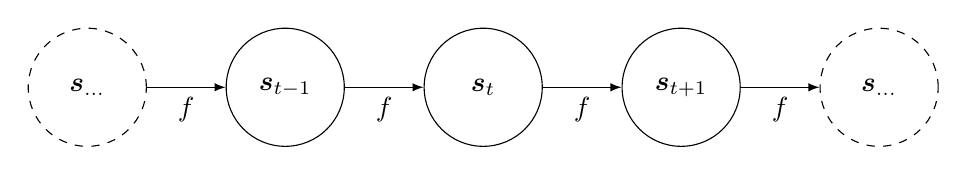
\begin{tikzpicture}[
        unit/.style={draw, circle, minimum size=1.5cm}]
        ]
        \node[unit, dashed] at (0,0) (a) {$\bm s_{\dots}$};
        \node[unit,right=of a] (b) {$\bm s_{t-1}$};
        \node[unit,right=of b] (c) {$\bm s_{t}$};
        \node[unit,right=of c] (d) {$\bm s_{t+1}$};
        \node[unit, dashed,right=of d] (e) {$\bm s_{\dots}$};

        \begin{scope}[->,>=latex]
          \draw (a) -- node[below] {$f$} (b);
          \draw  (b) -- node[below] {$f$} (c);
          \draw  (c) -- node[below] {$f$} (d);
          \draw (d) -- node[below] {$f$} (e);
      \end{scope}
      \end{tikzpicture}
    \end{figure}}
  \end{itemize}

\end{frame}

\begin{frame}
  \frametitle{Dynamical system driven by external signal}
  \pause
  The state $\bm s_{t}$ of a dynamical system driven by an external signal $\bm x_{t}$ can be described by\pause

  
  \begin{equation}
    \bm s_{t} \pause = f(\bm s_{t-1};\bm x_{t}; \bm\theta)
  \end{equation}
  \pause

  \begin{itemize}
  \item the state $\bm s _{t}$ includes information about the entire past sequence
  \item the unfolded computational graph: \pause
    \visible<+->{
        \begin{figure}[h!]
      \centering
      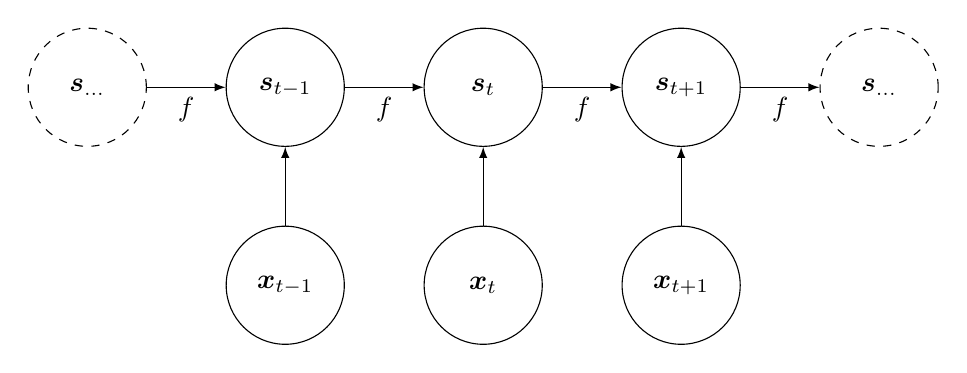
\begin{tikzpicture}[
        unit/.style={draw, circle, minimum size=1.5cm}]
        ]
        \node[unit, dashed] at (0,0) (a) {$\bm s_{\dots}$};
        \node[unit,right=of a] (b) {$\bm s_{t-1}$};
        \node[unit,right=of b] (c) {$\bm s_{t}$};
        \node[unit,right=of c] (d) {$\bm s_{t+1}$};
        \node[unit, dashed,right=of d] (e) {$\bm s_{\dots}$};

        \begin{scope}[->,>=latex]
          \draw (a) -- node[below] {$f$} (b);
          \draw (b) -- node[below] {$f$} (c);
          \draw (c) -- node[below] {$f$} (d);
          \draw (d) -- node[below] {$f$} (e);
        \end{scope}

        \node[unit,below=of b] (x1) {$\bm x_{t-1}$};
        \node[unit,below=of c] (x2) {$\bm x_{t}$};
        \node[unit,below=of d] (x3) {$\bm x_{t+1}$};

        \begin{scope}[->,>=latex]
          \draw (x1) --   (b);
          \draw (x2) --  (c);
          \draw (x3) --  (d);
        \end{scope}

      \end{tikzpicture}
    \end{figure}}
  \end{itemize}
\end{frame}

\begin{frame}
  \frametitle{Recurrent neural networks as sequence models}
  \pause
  \begin{itemize}
  \item Dynamical systems are sequences (temporal, etc)\pause
  \item Recurrence relations can be modeled by \textit{recurrent} neural networks (RNNs) \pause
  \item In an RNN, hidden units $\bm h$ represent the state $\bm s$ of the system: \pause
    \begin{equation}
      \bm h_{t} = \pause f(\bm h_{t-1}, \bm x_{t};\bm \theta)
    \end{equation}
    \pause
                \visible<+->{\begin{figure}[h!]
      \centering
      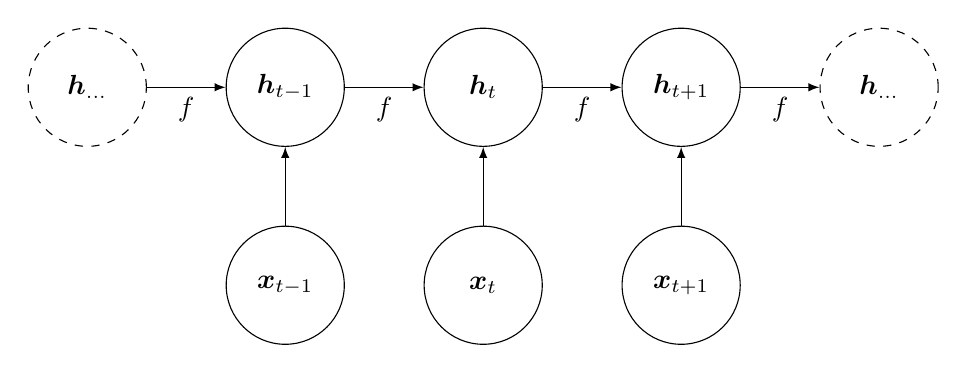
\begin{tikzpicture}[
        unit/.style={draw, circle, minimum size=1.5cm}]
        ]
        \node[unit, dashed] at (0,0) (a) {$\bm h_{\dots}$};
        \node[unit,right=of a] (b) {$\bm h_{t-1}$};
        \node[unit,right=of b] (c) {$\bm h_{t}$};
        \node[unit,right=of c] (d) {$\bm h_{t+1}$};
        \node[unit, dashed,right=of d] (e) {$\bm h_{\dots}$};

        \begin{scope}[->,>=latex]
          \draw (a) -- node[below] {$f$} (b);
          \draw (b) -- node[below] {$f$} (c);
          \draw (c) -- node[below] {$f$} (d);
          \draw (d) -- node[below] {$f$} (e);
        \end{scope}

        \node[unit,below=of b] (x1) {$\bm x_{t-1}$};
        \node[unit,below=of c] (x2) {$\bm x_{t}$};
        \node[unit,below=of d] (x3) {$\bm x_{t+1}$};

        \begin{scope}[->,>=latex]
          \draw (x1) --   (b);
          \draw (x2) --  (c);
          \draw (x3) --  (d);
        \end{scope}

      \end{tikzpicture}}
    \end{figure}
  \end{itemize}
\end{frame}

\begin{frame}
  \frametitle{Computational advantages of RNN}
  \pause

  \begin{itemize}
  \item Transition function $f$ maps past variable-length sequence
    $(\bm x_{t}, \bm x_{t-1}, \bm x^{(t-2)}, \ldots, \bm x^{(2)}, \bm x^{(1)})$ to fixed-length state $\bm h_{t}$ \pause
  \item Model always has same input size $\bm h_{t-1}$ \pause
  \item Single function $f$ with same parameters operates on all time steps \pause
  \item Further architectural features (including output layers) use information from $\bm h$ to make predictions
  \end{itemize}
  \pause

  \begin{figure}[h!]
    \centering
    \visible<+->{
      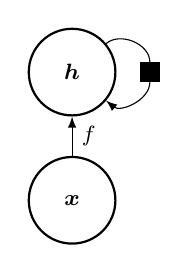
\begin{tikzpicture}[%baseline,
        unit/.style={draw, circle, node distance=.5cm, minimum size=1.1cm, font={\footnotesize}, thick}]
        ]
        \node[unit] at (0,0) (h) {$\bm h$};
        \node[unit,below=of h] (x) {$\bm x$};
        \node[draw,rectangle,fill,black,right=3mm of h] (t) {};
        \begin{scope}
          \draw[->,>=latex] (x) -- node[right] {\footnotesize$f$} (h);
          \draw (h) edge [out=40, in=90] (t);
          \draw[->,>=latex] (t) edge [out=270, in=320] (h);
        \end{scope}        
      \end{tikzpicture}
      }
    \visible<+->{
      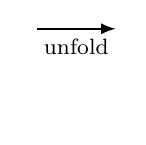
\begin{tikzpicture}%[baseline]
        \node at (0,0) {};
        \draw[thick,->,>=latex] (0,1) -- node[below]{\footnotesize unfold} (1,1);
      \end{tikzpicture}}
    \visible<+->{
      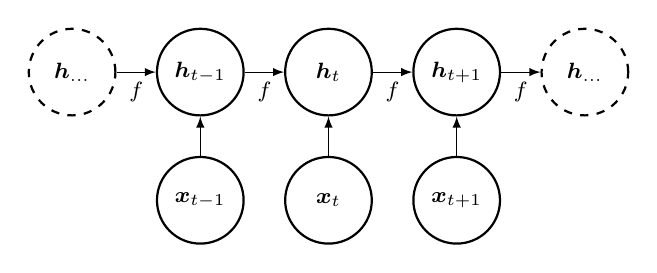
\begin{tikzpicture}[%baseline,
        unit/.style={draw, circle, node distance=.5cm, minimum size=1.1cm, font={\footnotesize}, thick}]
        ]
        \node[unit, dashed] at (0,0) (a) {$\bm h_{\dots}$};
        \node[unit,right=of a] (b) {$\bm h_{t-1}$};
        \node[unit,right=of b] (c) {$\bm h_{t}$};
        \node[unit,right=of c] (d) {$\bm h_{t+1}$};
        \node[unit, dashed,right=of d] (e) {$\bm h_{\dots}$};

        \begin{scope}[->,>=latex]
          \draw (a) -- node[below] {\footnotesize$f$} (b);
          \draw (b) -- node[below] {\footnotesize$f$} (c);
          \draw (c) -- node[below] {\footnotesize$f$} (d);
          \draw (d) -- node[below] {\footnotesize$f$} (e);
        \end{scope}

        \node[unit,below=of b] (x1) {$\bm x_{t-1}$};
        \node[unit,below=of c] (x2) {$\bm x_{t}$};
        \node[unit,below=of d] (x3) {$\bm x_{t+1}$};

        \begin{scope}[->,>=latex]
          \draw (x1) --   (b);
          \draw (x2) --  (c);
          \draw (x3) --  (d);
        \end{scope}

      \end{tikzpicture}}
    \visible<+->{\caption{Recurrent network with no outputs. L: recurrent graph; R: time-unfolded computational graph. (Black square indicates time-step-delayed interaction)}}
    \end{figure}
  \end{frame}



  

  \begin{frame}
    \frametitle{RNN models for sequence tasks}
    \pe

    \begin{itemize}
    \item \textbf{Generation} (\texttt{Vec2Seq}): $f_{\bm\th} : \mb R^{D}\to \mb R^{N_{\infty}C}$\pe
      \begin{itemize}
      \item Input: vector of size $D$\pe
      \item Output: arbitrary-length sequence of size $C$ vectors\pe
      \item Applications: language modeling, image captioning
      \end{itemize}
    \item \textbf{Classification} (\texttt{Seq2Vec}): $f_{\bm\th}: \mb R^{TD} \to \mb R^{C}$ \pe
      \begin{itemize}
      \item Input: variable-length sequence\pe       
      \item Output: fixed-length output vector (e.g.\ class label)\pe
      \end{itemize}
    \item \textbf{Translation} (\texttt{Seq2Seq}):  $f_{\bm\th}: \mb R^{TD} \to \mb R^{T'C}$ \pe
      \begin{itemize}
      \item Aligned case: $T=T'$\pe
      \item Unaligned case: $T\ne T'$\pe
      \item Application: neural machine translation
      \end{itemize}
    \end{itemize}
  \end{frame}
  

\section{Vec2Seq}
\begin{frame}
  \frametitle{Vec2Seq model for sequence generation}
  \pe
  Vec2Seq models map a fixed-length vector $\bm x\in\mb R^D$ onto a distribution over sequences $\bm Y\in \mb R^{T\times C}$ (or, $\bm y_{1:T}\in \bm R^{C}$; that is, $T$ sequences, with each $y_t$ a vector of length $C$)\pe

  \medskip
  Thus, the generative model is given by:
  \begin{equation}
    p(\bm y_{1:T}|\bm x) = \sum _{\bm h_{1:T}}p(\bm y_{1:T}, \bm h_{1:T}|\bm x)
  \end{equation}\pe
  where  $\bm h_{t}$ is the hidden state of the model.\pe

  By the multiplication rule, we can write:\pe
  \begin{equation}
    \sum _{\bm h_{1:T}}p(\bm y_{1:T}, \bm h_{1:T}|\bm x) \pe =
    \sum_{\bm h_{1:T}}\prod_{t=1}^{T} p(\bm y_{t}|\bm h_{t})p(\bm h_{t}|\bm h_{t-1}, \bm y_{t-1}, \bm x)
  \end{equation}
  \begin{itemize}
  \item Initial hidden state: \pe $p(\bm h_{1}|\bm h_{0},\bm y_{0},\bm x) = p(\bm h_{1}|\bm x)$\pe
  \end{itemize}
\end{frame}

\begin{frame}
  \frametitle{Vec2Seq model (cont.)}
  \pe
  The output distribution is given by:
  \begin{equation}
    p(\bm y_{t}|\bm h_{t}) =
    \begin{cases}
      \text{Cat}(\bm y_{t}|\mc{S}(\bm W_{ho}\bm h_{t} + \bm b_{o})) , & \text{(qualitative outputs)} \\[2mm]
      \mc{N}(\bm y_{t}|\bm W_{ho}\bm h_{t} + \bm b_{o}, \sigma^{2}\bm I), & \text{(real-valued outputs)}
    \end{cases}
  \end{equation}

  \pe 
  \begin{itemize}
  \item $\bm W_{ho}$: matrix of hidden--output weights\pe
  \item $\bm b_o$: bias term\pe
  \item $\bm y_t$ is the observed vector, while $\bm o_t$ is the predicted value (using NN notation)
  \end{itemize}
  \pe
  The hidden state is typically deterministic: \pe
  \begin{equation}
    \bm h_{t} = \varphi(\bm W_{xh}[\bm x;\bm o_{t-1}] + \bm W_{hh}\bm h_{t-1} + \bm b_{h})
  \end{equation}  \pe
  \begin{itemize}
  \item $\bm W_{xh}$: input--hidden weight matrix\pe
  \item  $\bm W_{hh}$: hidden--hidden weight matrix\pe
  \item $\bm b_h$: bias term
  \end{itemize}
\end{frame}

\begin{frame}
  \frametitle{Vec2Seq RNN: circuit diagram and computation graph}
  \pe
    \begin{figure}[h!]
    \centering
    \visible<+->{
      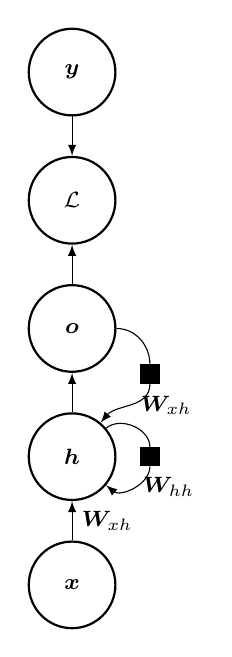
\begin{tikzpicture}[%baseline,
        unit/.style={draw, circle, node distance=.5cm, minimum size=1.1cm, font={\footnotesize}, thick}]
        ]
        \node[unit] at (0,0) (h) {$\bm h$};
        \node[unit,below=of h] (x) {$\bm x$};
        \node[unit,above=of h] (o) {$\bm o$};
        \node[unit,above=of o] (l) {$\mc L$};
        \node[unit,above=of l] (y) {$\bm y$};        
        \node[draw,rectangle,fill,black,right=3mm of h] (t) {};
        \node[draw,rectangle,fill,black,above=8mm of t] (u) {};        
        \begin{scope}
          \draw[->,>=latex] (x) -- node[right] {\footnotesize$\bm W_{xh}$} (h); 
          \draw (h) edge [out=40, in=90] (t);
          \draw[->,>=latex] (t) edge [out=270, in=320] node[right]  {\footnotesize$\bm W_{hh}$} (h);
          \draw (o) edge [out=0, in=90] (u);
          \draw[->,>=latex] (u) edge [out=270, in=50]  node[right]  {\footnotesize$\bm W_{xh}$} (h);
          \draw[->,>=latex] (h) -- (o);
          \draw[->,>=latex] (o) -- (l);
          \draw[->,>=latex] (y) -- (l);
        \end{scope}        
      \end{tikzpicture}
      }
    \visible<+->{
      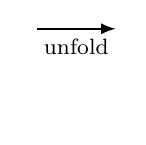
\begin{tikzpicture}%[baseline]
        \node at (0,0) {};
        \draw[thick,->,>=latex] (0,1) -- node[below]{\footnotesize unfold} (1,1);
      \end{tikzpicture}}
    \visible<+->{
      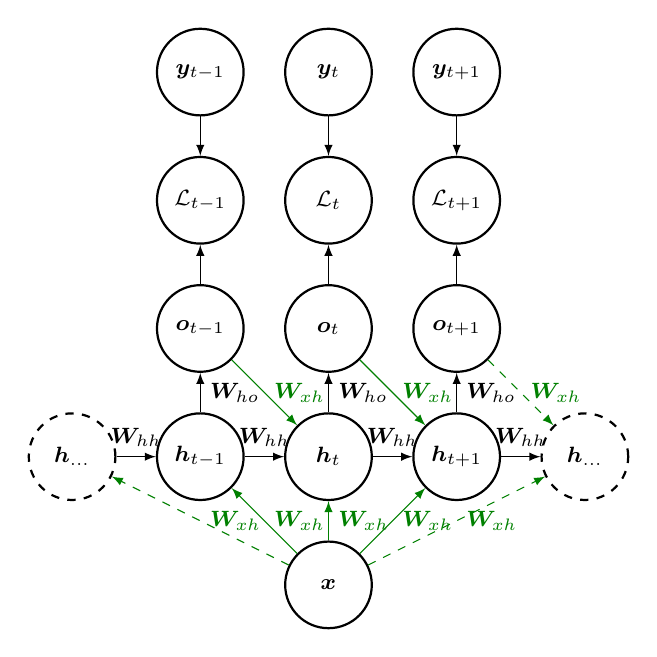
\begin{tikzpicture}[%baseline,
        unit/.style={draw, circle, node distance=.5cm, minimum size=1.1cm, font={\footnotesize}, thick}]
        ]
        \node[unit, dashed] at (0,0) (a) {$\bm h_{\dots}$};
        \node[unit,right=of a] (b) {$\bm h_{t-1}$};
        \node[unit,right=of b] (c) {$\bm h_{t}$};
        \node[unit,right=of c] (d) {$\bm h_{t+1}$};
        \node[unit, dashed,right=of d] (e) {$\bm h_{\dots}$};
        \node[unit, above=of b] (o1) {$\bm o_{t-1}$};
        \node[unit, above=of c] (o2) {$\bm o_{t}$};
        \node[unit, above=of d] (o3) {$\bm o_{t+1}$};
        \node[unit, above=of o1] (l1) {$\mc L_{t-1}$};
        \node[unit, above=of o2] (l2) {$\mc L_{t}$};
        \node[unit, above=of o3] (l3) {$\mc L_{t+1}$};
        \node[unit, above=of l1] (y1) {$\bm y_{t-1}$};
        \node[unit, above=of l2] (y2) {$\bm y_{t}$};
        \node[unit, above=of l3] (y3) {$\bm y_{t+1}$};        
        \begin{scope}[->,>=latex]
          \draw (a) -- node[above] {\footnotesize$\bm W_{hh}$} (b);
          \draw (b) -- node[above] {\footnotesize$\bm W_{hh}$} (c);
          \draw (c) -- node[above] {\footnotesize$\bm W_{hh}$} (d);
          \draw (d) -- node[above] {\footnotesize$\bm W_{hh}$} (e);
          \draw (b) -- node[right] {\footnotesize$\bm W_{ho}$} (o1);
          \draw (c) -- node[right] {\footnotesize$\bm W_{ho}$} (o2);
          \draw (d) -- node[right] {\footnotesize$\bm W_{ho}$} (o3);
        \end{scope}

        \node[unit,below=of c] (x) {$\bm x$};

       \begin{scope}[->,>=latex, green!50!black]
          \draw (x) -- node[right] {\footnotesize$\bm W_{xh}$}  (b);
          \draw (x) -- node[right] {\footnotesize$\bm W_{xh}$} (c);
          \draw (x) -- node[right] {\footnotesize$\bm W_{xh}$} (d);
          \draw[dashed] (x) -- node[right] {\footnotesize$\bm W_{xh}$} (a);
          \draw[dashed] (x) -- node[right] {\footnotesize$\bm W_{xh}$} (e); 
          \draw (o1) -- node[right] {\footnotesize$\bm W_{xh}$} (c);
          \draw (o2) -- node[right] {\footnotesize$\bm W_{xh}$} (d);
          \draw [dashed] (o3) -- node[right] {\footnotesize$\bm W_{xh}$} (e);
        \end{scope}

        
        \begin{scope}[->,>=latex]
          \draw (o1) -- (l1);
          \draw (o2) -- (l2);
          \draw (o3) -- (l3);          
          \draw (y1) -- (l1);
          \draw (y2) -- (l2);
          \draw (y3) -- (l3);          
        \end{scope}

      \end{tikzpicture}}
  %  \visible<+->{\caption{Recurrent network with no outputs. L: recurrent graph; R: time-unfolded computational graph. (Black square indicates time-step-delayed interaction)}}
    \end{figure}
  \end{frame}


  \begin{frame}
    \frametitle{Vec2Seq model summary}
    \pe
      \begin{minipage}{.15\linewidth}
    \visible<+->{
      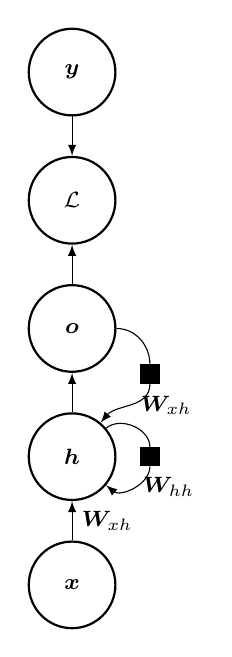
\begin{tikzpicture}[%baseline,
        unit/.style={draw, circle, node distance=.5cm, minimum size=1.1cm, font={\footnotesize}, thick}]
        ]
        \node[unit] at (0,0) (h) {$\bm h$};
        \node[unit,below=of h] (x) {$\bm x$};
        \node[unit,above=of h] (o) {$\bm o$};
        \node[unit,above=of o] (l) {$\mc L$};
        \node[unit,above=of l] (y) {$\bm y$};        
        \node[draw,rectangle,fill,black,right=3mm of h] (t) {};
        \node[draw,rectangle,fill,black,above=8mm of t] (u) {};        
        \begin{scope}
          \draw[->,>=latex] (x) -- node[right] {\footnotesize$\bm W_{xh}$} (h); 
          \draw (h) edge [out=40, in=90] (t);
          \draw[->,>=latex] (t) edge [out=270, in=320] node[right]  {\footnotesize$\bm W_{hh}$} (h);
          \draw (o) edge [out=0, in=90] (u);
          \draw[->,>=latex] (u) edge [out=270, in=50]  node[right]  {\footnotesize$\bm W_{xh}$} (h);
          \draw[->,>=latex] (h) -- (o);
          \draw[->,>=latex] (o) -- (l);
          \draw[->,>=latex] (y) -- (l);
        \end{scope}        
      \end{tikzpicture}
      }
  \end{minipage}\hfill
  \begin{minipage}{.8\linewidth}
    \pe
    Update equations:
    \begin{eqnarray}
      \bm a_{t} &=& \bm W_{xh}[\bm x;\bm o_{t-1}] + \bm W_{hh}\bm h_{t-1} + \bm b_{h}\\\pe
      \bm h_{t} &=&  \varphi(\bm a_{t})\\\pe
      \bm o_t &=& \pe \bm W_{oh}\bm h_t + \bm b_o \\\pe
      \bm \hat{\bm y}_t &=& \mc{S}(\bm o_t)
    \end{eqnarray}
    \pe
    \begin{itemize}
    \item In typical applications, $\bm o_t = [o_{t1},o_{t2},\ldots,o_{tC}]$ (e.g.\ one-hot vector, each representing a character)\pe
    \item $\bm o_t$ depends on $\bm h_t$, which depends on $\bm o_{t-1}$\pe
    \item $\bm o_t$ depends on \textit{all} past observations and the fixed input $\bm x$ \pe
    \item $[\bm x;\bm o_{t-1}]$ denotes the stacking of $\bm x$ and $\bm o_{t-1}$\pe
    \item So, if $\bm x\in\mb R^D$, $\bm o_t\in\mb R^C$, and $\bm h_t\in\mb R^M$, then $\bm W_{xh}\in \mb R^{(D+C)\times M}$\pe
    \item $M$ is the number of units (neurons) in the hidden layer
    \end{itemize}
  \end{minipage}
  \end{frame}


    \begin{frame}
    \frametitle{Application: image captioning}
    \pe
    Image or processed version from CNN is used as input, with output as sequence of descriptive words \pe
      \begin{center}
        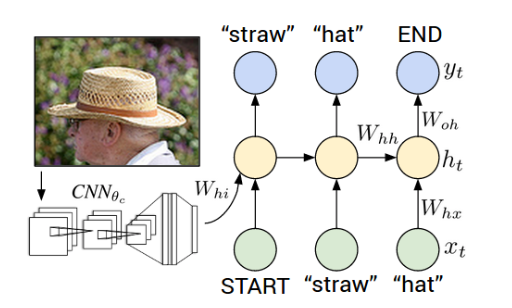
\includegraphics[width=.7\textwidth]{image-captioning}

        {\tiny Source: \url{https://towardsdatascience.com/image-captioning-in-deep-learning-9cd23fb4d8d2}}
      \end{center}
    \end{frame}
    
\section{Seq2Seq}
\begin{frame}
  \frametitle{Seq2Seq model: aligned case}\pe
  Seq2seq models map a sequence of vectors $\bm x_{1:T}\in\mb R^D$ onto another sequence $\bm y_{1:T’}\in \mb R^C$. \pe
  We consider the aligned case (dense sequence modeling) where $T = T’$:
  \begin{equation}
    p(\bm y_{1:T}|\bm x_{1:T}) = \pe\sum_{\bm h_{1:T}}\prod_{t=1}^Tp(\bm y_t|\bm h_t) \mb I(\bm h_t = f(\bm h_{t-1},\bm x_t))
  \end{equation}
  \pe where the initial hidden state is $\bm h_1 = f(\bm h_0,\bm x_1) = f_0(\bm x_1)$.\pe
  \begin{itemize}
  \item The hidden state is given by:\pe
    \begin{equation}
      \bm h_t  = \varphi(\bm W_{xh}\bm h_t + \bm W_{hh}\bm h_{t-1} + \bm h)
    \end{equation}
    \pe
  \item The output is given by:\pe
    \begin{equation}
      \bm o_t = \bm W_{ho}\bm h_t + \bm b_o
    \end{equation}
  \end{itemize}
\end{frame}
\begin{frame}
  \frametitle{Aligned seq2seq circuit diagram}
  \pause
  \begin{minipage}{.15\linewidth}
    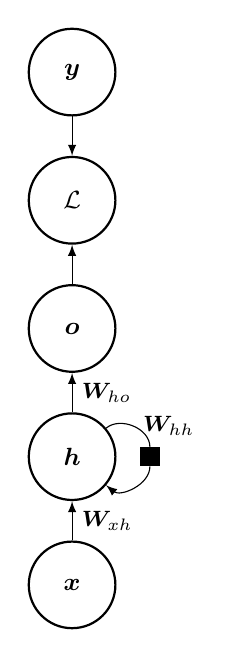
\begin{tikzpicture}[%baseline,
      unit/.style={draw, circle, node distance=.5cm, minimum size=1.1cm, font={\small}, thick}]
      ]
      \node[unit] at (0,0) (h) {$\bm h$};
      \node[unit,below=of h] (x) {$\bm x$};
      \node[unit,above=of h] (o) {$\bm {o}$};
      \node[unit,above=of o] (l) {$\mc L$};
      \node[unit,above=of l] (y) {$\bm y$};
      \node[draw,rectangle,fill,black,right=3mm of h] (t) {};
      \begin{scope}
        \draw[->,>=latex] (x) -- node[right] {\footnotesize$\bm W_{xh}$} (h);
        \draw (h) edge [out=40, in=90] node[right] {\footnotesize$\bm W_{hh}$} (t);
        \draw[->,>=latex] (t) edge [out=270, in=320] (h);
        \draw[->,>=latex] (h) -- node[right] {\footnotesize $\bm W_{ho}$} (o);
        \draw[->,>=latex] (o) -- (l);
        \draw[->,>=latex] (y) --  (l) ;
      \end{scope}        
    \end{tikzpicture}
  \end{minipage}\hfill
  \begin{minipage}{.8\linewidth}
    The update equations for a seq2seq RNN are given by\pause
    \begin{eqnarray}
      \bm a_{t} &=& \bm b_h + \bm W_{hh} \bm h_{t-1} + \bm W_{xh} \bm x_{t} \\\pause
      \bm h_{t} &=& \tanh(\bm a_{t}) \\\pause
      \bm {o}_{t} &=& \bm b_o + \bm W_{ho}\bm h_{t}
    \end{eqnarray}     \pause
    \vspace{-3ex}
    \begin{itemize}
    \item $\bm x$: input sequence
    \item $\bm h$: hidden units
    \item $\bm b_h$, $\bm b_o$: bias vectors
    \item $\bm W_{xh}$: weight matrix of input--hidden unit connections
    \item $\bm W_{hh}$: weight matrix of hidden--hidden unit connections
    \item $\bm W_{ho}$: weight matrix of hidden--output unit connections
    \item $\bm {o}$: output vector 
    \item $\bm y$ target sequence
    \item $\mc L$: loss function measuring error between $\bm{\hat y}$ and $\bm y$
    \end{itemize}
  \end{minipage}

\end{frame}

\begin{frame}
  \frametitle{Seq2seq model: unaligned case}
  \pe
  \begin{minipage}{.5\linewidth}
  To map a sequence of length $T$ to another of length $T’$, we use an \textbf{encoder-decoder architecture}:\pe
  \begin{itemize}
  \item The encoder $f_e$ maps the input sequence onto a context vector
    \begin{equation}
      \bm c = f_e(\bm x_{1:T})
    \end{equation}
    \pe
  \item The decoder $f_d$ generates the output sequence by mapping from the context vector:\pe
    \begin{equation}
      \bm y_{1:T’} = f_d(\bm c)
    \end{equation}
  \end{itemize}
\end{minipage}\pe
\begin{minipage}{.45\linewidth}
  \begin{center}
    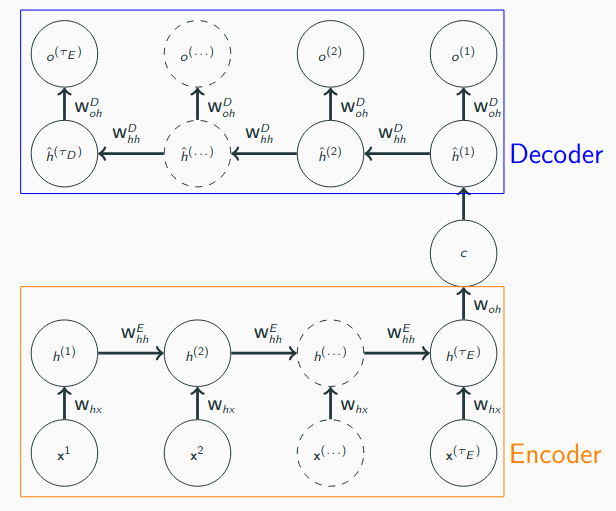
\includegraphics[width=.9\textwidth]{enc-dec-rnn}

    {\tiny Source: \url{https://www.inf.ed.ac.uk/teaching/courses/mlp/2019-20/lectures/mlp09-rnn.pdf}}
  \end{center}
\end{minipage}

\end{frame}


\begin{frame}
  \frametitle{Illustration of seq2seq for translation}\pe

  \begin{center}
    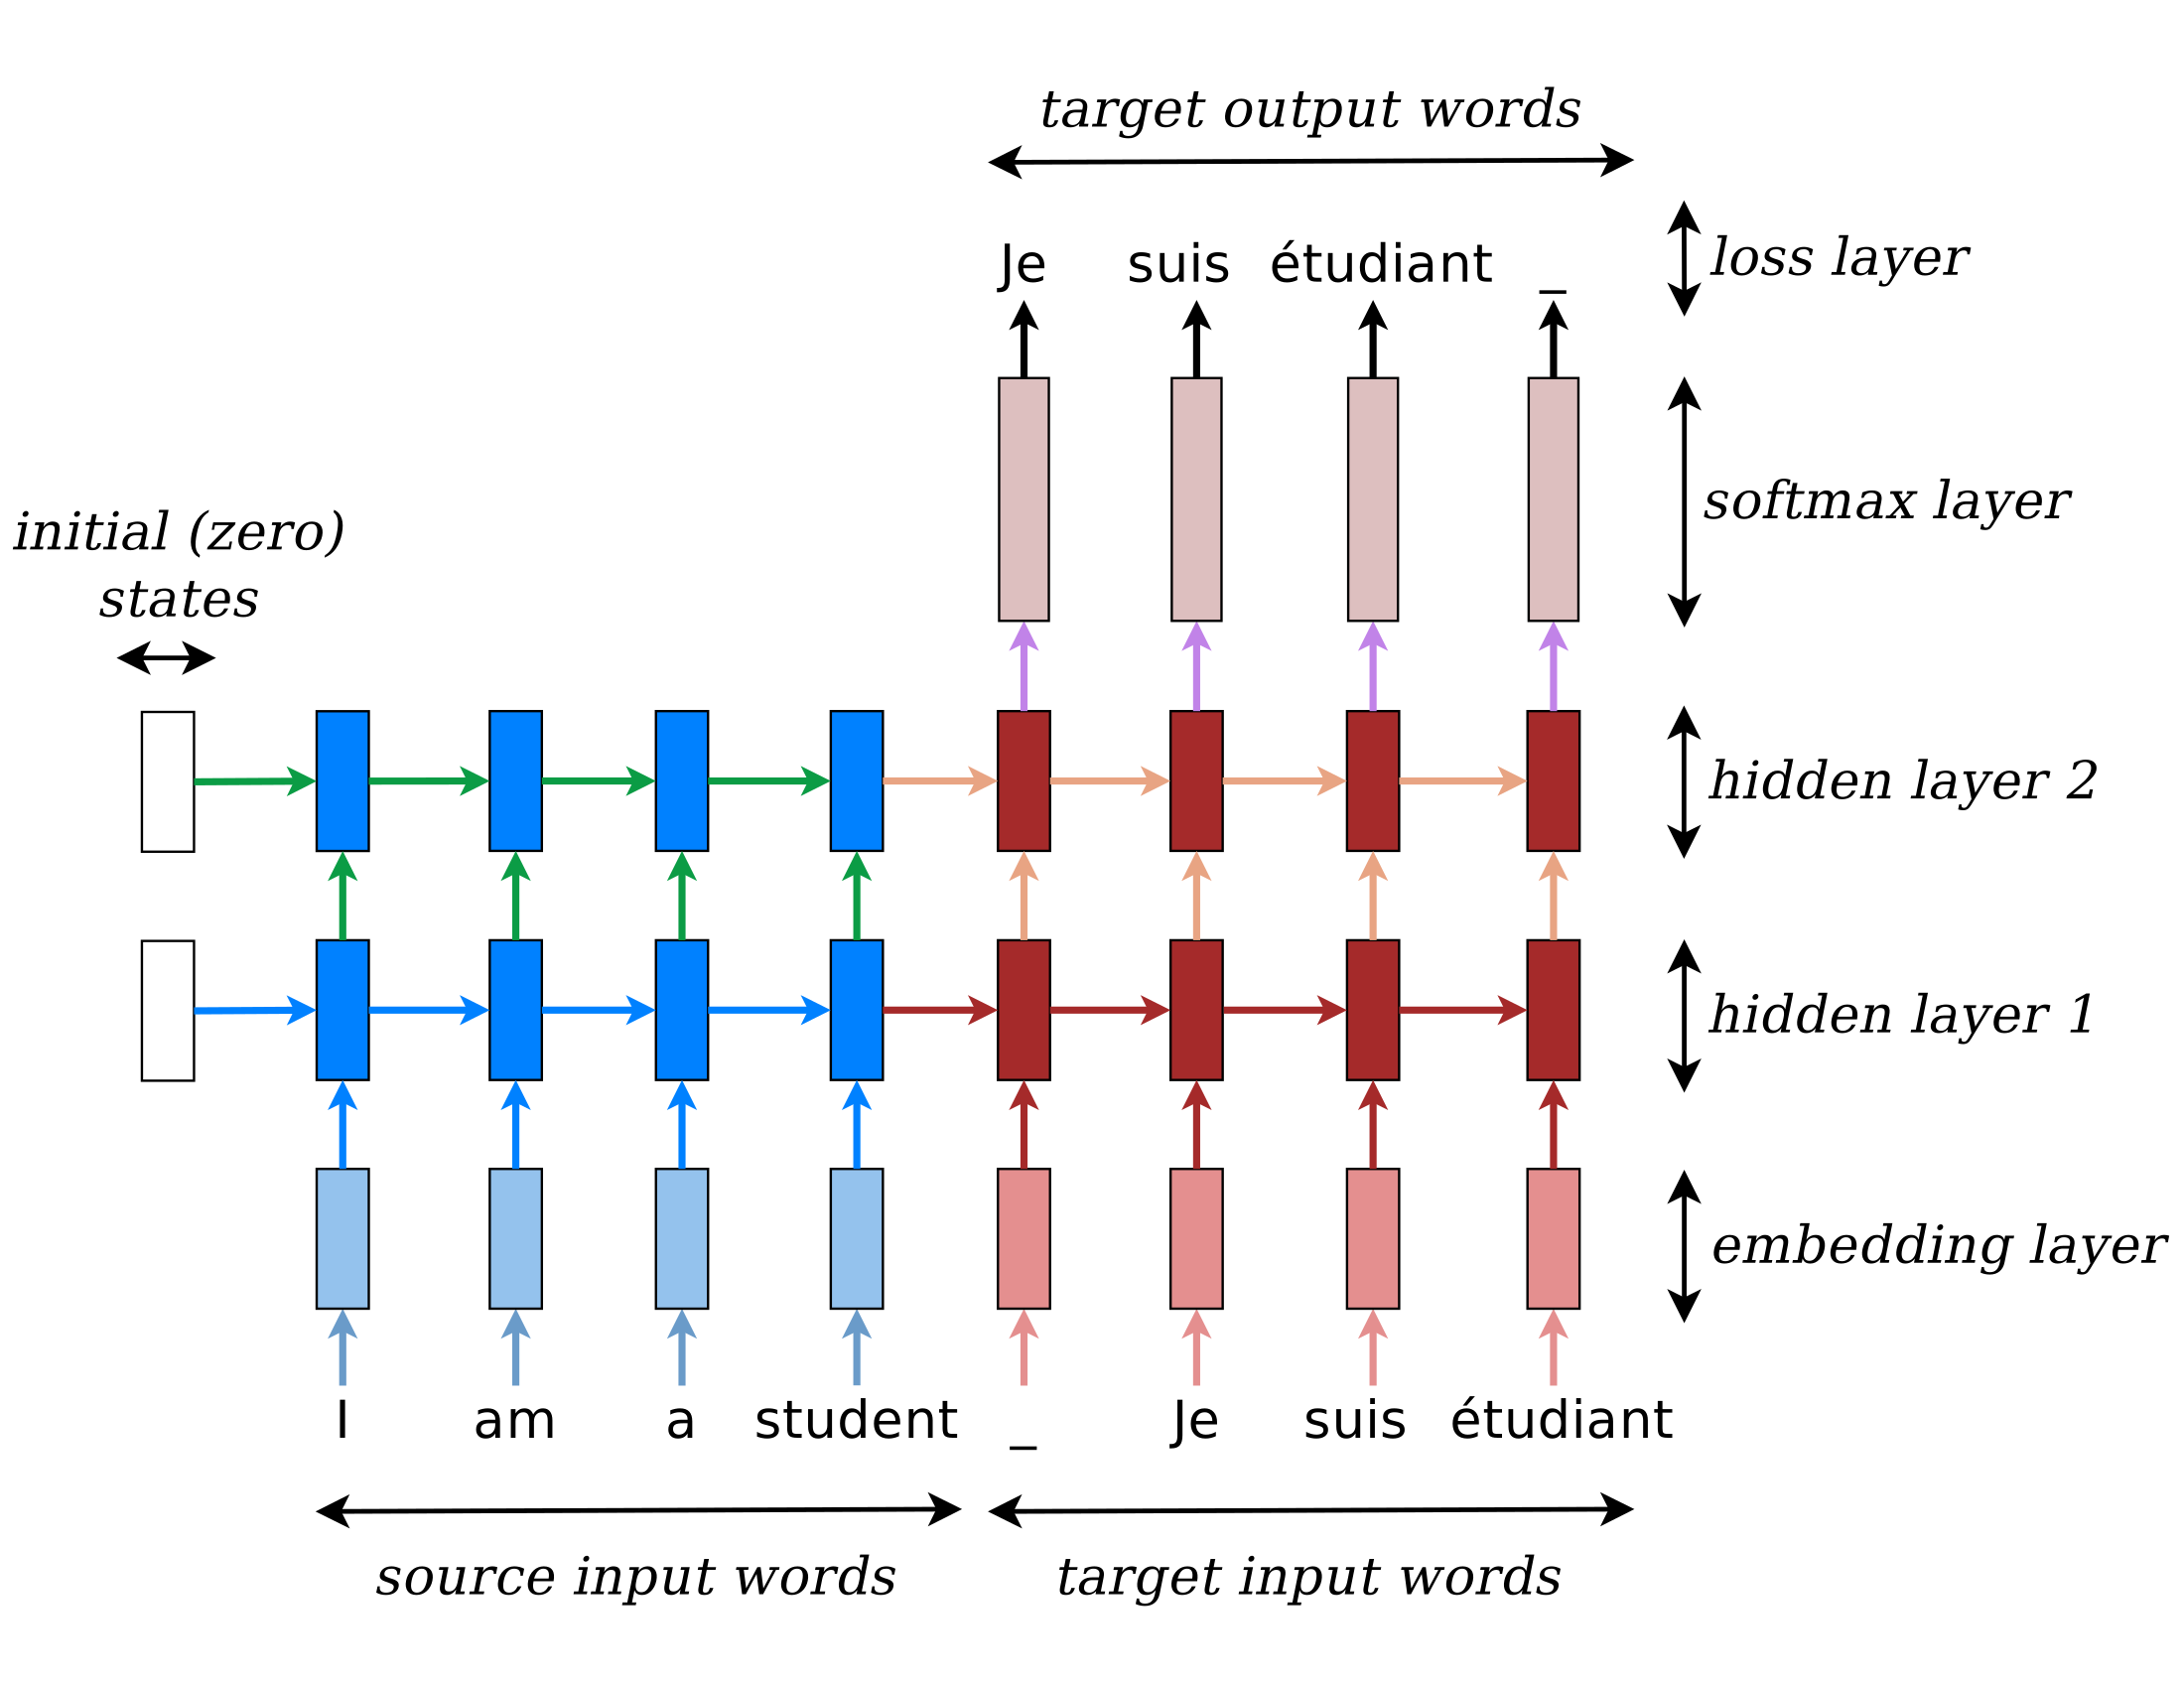
\includegraphics[width=.7\textwidth]{probml-seq2seq}

    Illustration of seq2seq model for English-to-French translation.

    {\tiny Source: \url{https://github.com/probml/pml-book/blob/main/book1-figures/Figure_15.8_A.png}}
  \end{center}

  

\end{frame}
\begin{frame}
  \frametitle{Deep RNNs}
  \pe
  More complex models can be developed by stacking \textbf{hidden chains}.\pe

  \begin{center}
    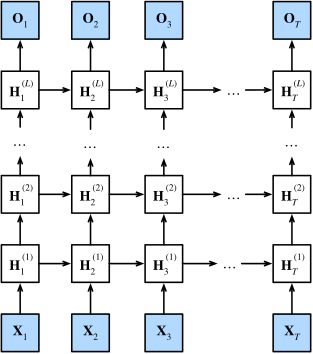
\includegraphics[width=.3\textwidth]{deep-rnn}

    {\tiny Source: \url{https://d2l.ai/chapter_recurrent-modern/deep-rnn.html}}
  \end{center}
  \pe
  
  The hidden state for layer $\ell$ at time $t$ is then given by:\pe
  \begin{equation}
    \bm h_t^{\ell}  = \varphi(\bm W_{xh}^{\ell}\bm h_t^{\ell-1} + \bm W_{hh}^{\ell}\bm h_{t-1}^{\ell} + \bm h^{\ell})
  \end{equation}
  \pe
  And the output at each time step as:\pe
  \begin{equation}
    \bm o_t = \bm W_{ho}\bm h_t^{L} + \bm b_o
  \end{equation}
  
\end{frame}


\section{Seq2Vec}
\begin{frame}
  \frametitle{Seq2vec models for sequence classification}
  \pe
  Seq2vec models map a sequence $\bm x_{1:T}\in\mb R^{D}$ onto a fixed length vector $\bm y\in\mb R^{C}$ (e.g.\ class label) \pe

  In the simple approach, the output depends on final state only. \pe
  
  Thus, the model can be specified as:\pe
  \begin{equation}
    p(y|\bm x_{1:T}) = \text{Cat}(y|\mc{S}(\bm W\bm h_{T})
  \end{equation}
  \pe
  where $\bm h_{T}$ is the final state of the RNN
  \pe

    \begin{center}
    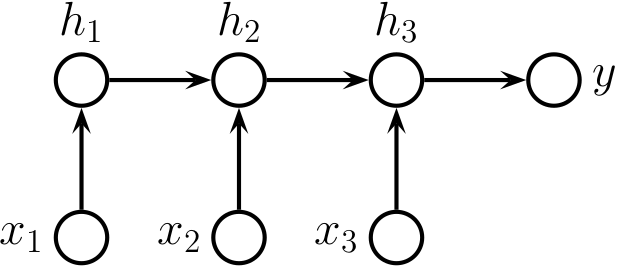
\includegraphics[width=.5\textwidth]{seq2veqsimple}

    % {\tiny Source: \url{https://d2l.ai/chapter_recurrent-modern/deep-rnn.html}}
  \end{center}
  
 \end{frame}

\begin{frame}
  \frametitle{Bidirectional seq2vec model}

  Bidirectional models allow the output to depend on the entire sequence (i.e.\ the hidden state depends on past and future contexts): \pe
  
  \begin{eqnarray}
    \bm h_{t}^{\to} &=& \varphi(\bm W_{xh}^{\to}\bm x_{t} + \bm W_{hh}^{\to}\bm h_{t-1}^{\to} + \bm b_{h}^{\to})\\\pe
    \bm h_{t}^{\leftarrow} &=& \varphi(\bm W_{xh}^{\leftarrow}\bm x_{t} + \bm W_{hh}^{\leftarrow}\bm h_{t+1}^{\leftarrow} + \bm b_{h}^{\leftarrow})\pe
  \end{eqnarray}
  \pe
  \begin{itemize}
  \item State at time $t$: $\bm h_{t} = [\bm h_{t}^{\to},\bm h_{t}^{\leftarrow}]$ \pe
  \item Final classification then given by: \pe
    \begin{equation}
      p(y|\bm x_{1:T}) = \text{Cat}(y|\bm W\mc{S}(\overline{\bm h}))
    \end{equation}
    \pe
    where $\overline{\bm h} = \fr1T\sum_{t=1}^{T}\bm h_{t}$
  \end{itemize}
  \pe
  
    \begin{center}
    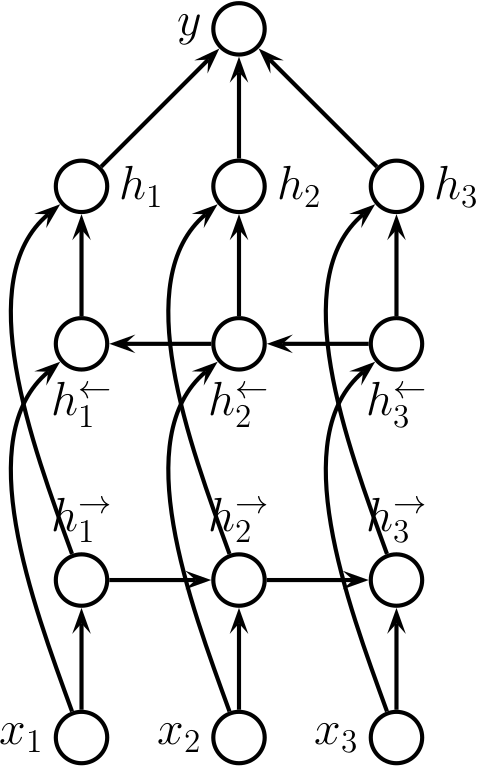
\includegraphics[width=.1\textwidth]{seq2veqbi}

    % {\tiny Source: \url{https://d2l.ai/chapter_recurrent-modern/deep-rnn.html}}
  \end{center}
  
\end{frame}
\section{Training}
\begin{frame}
  \frametitle{Long-term dependencies in RNNs}
  \pause
  \begin{itemize}
  \item RNNs involve multiple compositions of the same function, e.g.\ in a simple network: \pause
    \begin{equation}
      \bm{h}_{t} = \bm{W}^{T}\bm{h}_{t-1}
    \end{equation}
    \pause
  \item Given the above recurrence relation, we can then write:\pause
    \begin{eqnarray}
      \bm{h}_{t} &=& (\bm{W}^{t})^{T}\bm{h}^{(0)} \\\pause
      \bm{h}_{t} &=& \bm{Q}^{T}\bm{\Lambda}^{t}\bm{Q}\bm{h}^{(0)} 
    \end{eqnarray}
    \pause
    where $\bm\Lambda$ is a diagonal matrix of eigenvalues $\la_{i}$
    \pause
  \item Thus the eigenvalues are raised to the power of $t$\pause
    \begin{itemize}
    \item $\la_{i} < 1$: decay to zero (vanishing gradients)
    \item $\la_{i} > 1$: exploding gradients 
    \end{itemize}
  \end{itemize}
\end{frame}

\begin{frame}
  \frametitle{RNN considerations}
  \pause

  \begin{itemize}
  \item RNNs are fitted via the \textbf{backpropagation through time} (BPTT) algorithm
    \begin{itemize}
    \item computationally expensive
    \end{itemize}
    \pause
  \item Challenging to learn \textbf{long-term dependencies} due to vanishing/exploding gradients. \pause Strategies:
    \pause
    \begin{itemize}
    \item skip connections across time \pause
    \item leaky units across different time scales (via linear self-connections that weight information from the
      past)\pause
      \begin{equation}
        \bm{h}_{t} \leftarrow \alpha\bm{h}_{t-1} + (1-\alpha)\bm{h}_{t}
      \end{equation}\pause
      where $\alpha$ is the weight
      \item gradient clipping\pause
      \item train RNN to reset irrelevant states to zero at various points in sequence (via gated units)
      \end{itemize}
    \end{itemize}
    
  \end{frame}

  \section{LSTM}
\begin{frame} 
  \frametitle{Gated RNNs}
  \pause

  Gated RNNs are a generalization of leaky units that allow for time-dependent variation of self-connection
  weights. \pause
  \begin{itemize}
    \item In leaky units, the weights are either manually set or learned as parameters, in order to accumlate information
  \item Gated RNNs enable the ``forgetting'' of old states
  \item Most effective gated RNNs in use:\pause
    \begin{itemize}
    \item long short-term memory (LSTM); \href{http://www.bioinf.jku.at/publications/older/2604.pdf}{Hochreiter and
        Schmidhuber, 1997}\pause
    \item gated recurrent unit (GRU) \href{https://arxiv.org/pdf/1406.1078v3.pdf}{Cho et al., 2014}\pe
    \item   The LSTM cell has four neural network layers (compared to one layer in the standard RNN)        
    \end{itemize}
  \end{itemize}
 
  \pause
  \visible<+->{
  \begin{figure}
    \centering
    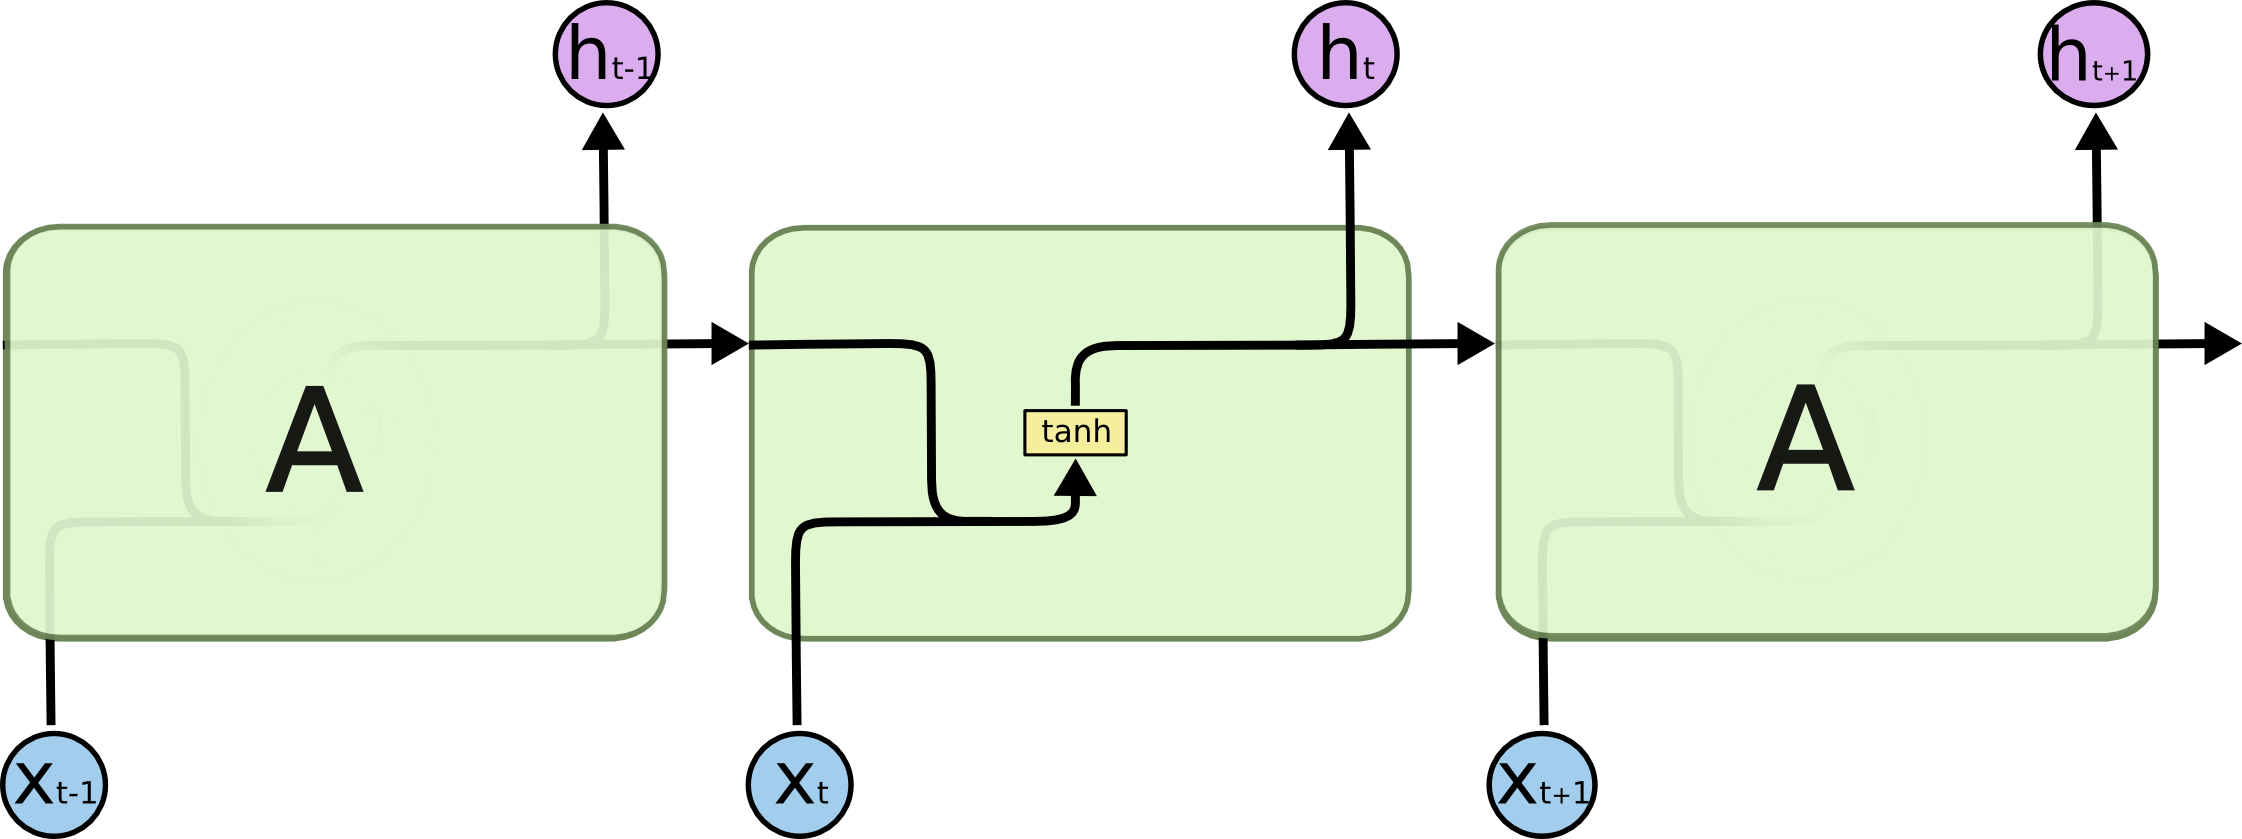
\includegraphics[width=.2\textwidth,trim={8.5cm 0 9.6cm 0}, clip]{LSTM3-SimpleRNN}\quad\quad\quad
    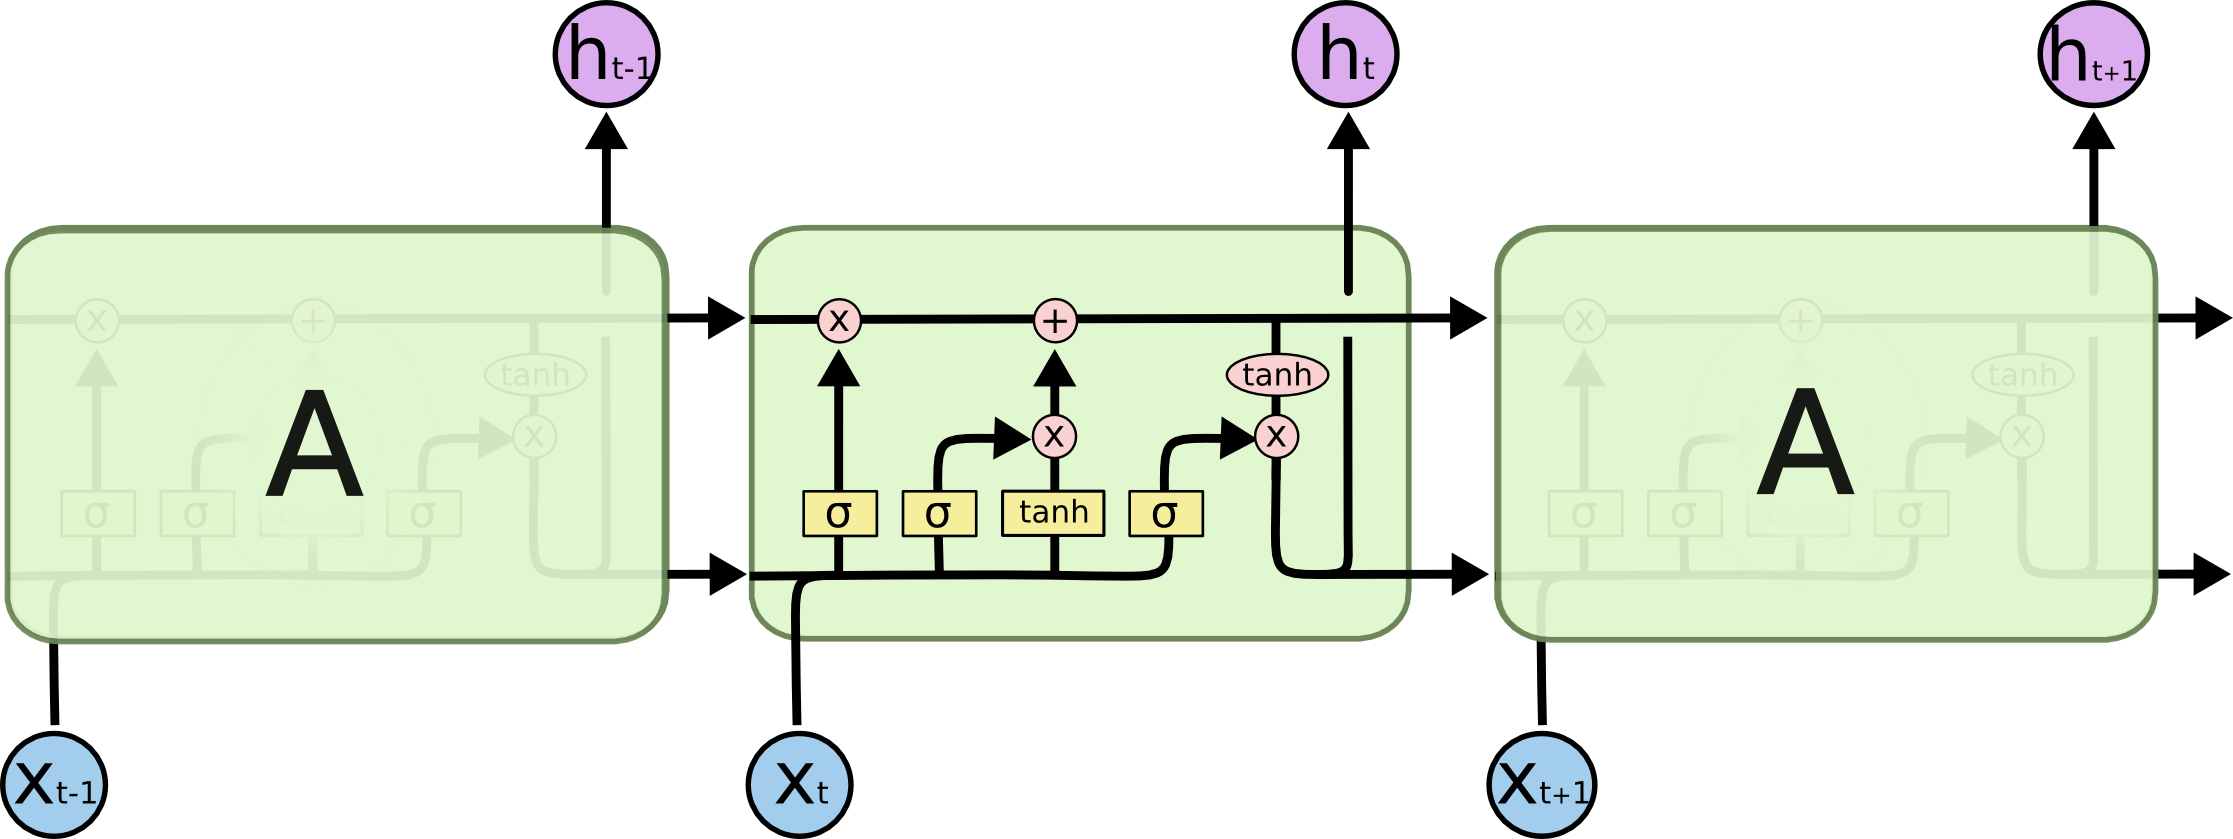
\includegraphics[width=.2\textwidth,trim={8.5cm 0 9.5cm 0}, clip]{LSTM3-chain}
    \caption{L: hidden unit in standard RNN; R: hidden unit in LSTM.
      
      {\tiny Source:
        \url{https://colah.github.io/posts/2015-08-Understanding-LSTMs/}}}
  \end{figure}}

\end{frame}
 

\begin{frame}
  \frametitle{LSTM chains and blocks}
  \pause

  \begin{itemize}
  %\item Weights and biases in LSTM networks are typically time-invariant (shared for different time steps)\pe
  \item There are as many LSTM cells are there are hidden units in current implementations\pe
    
    \begin{center}
      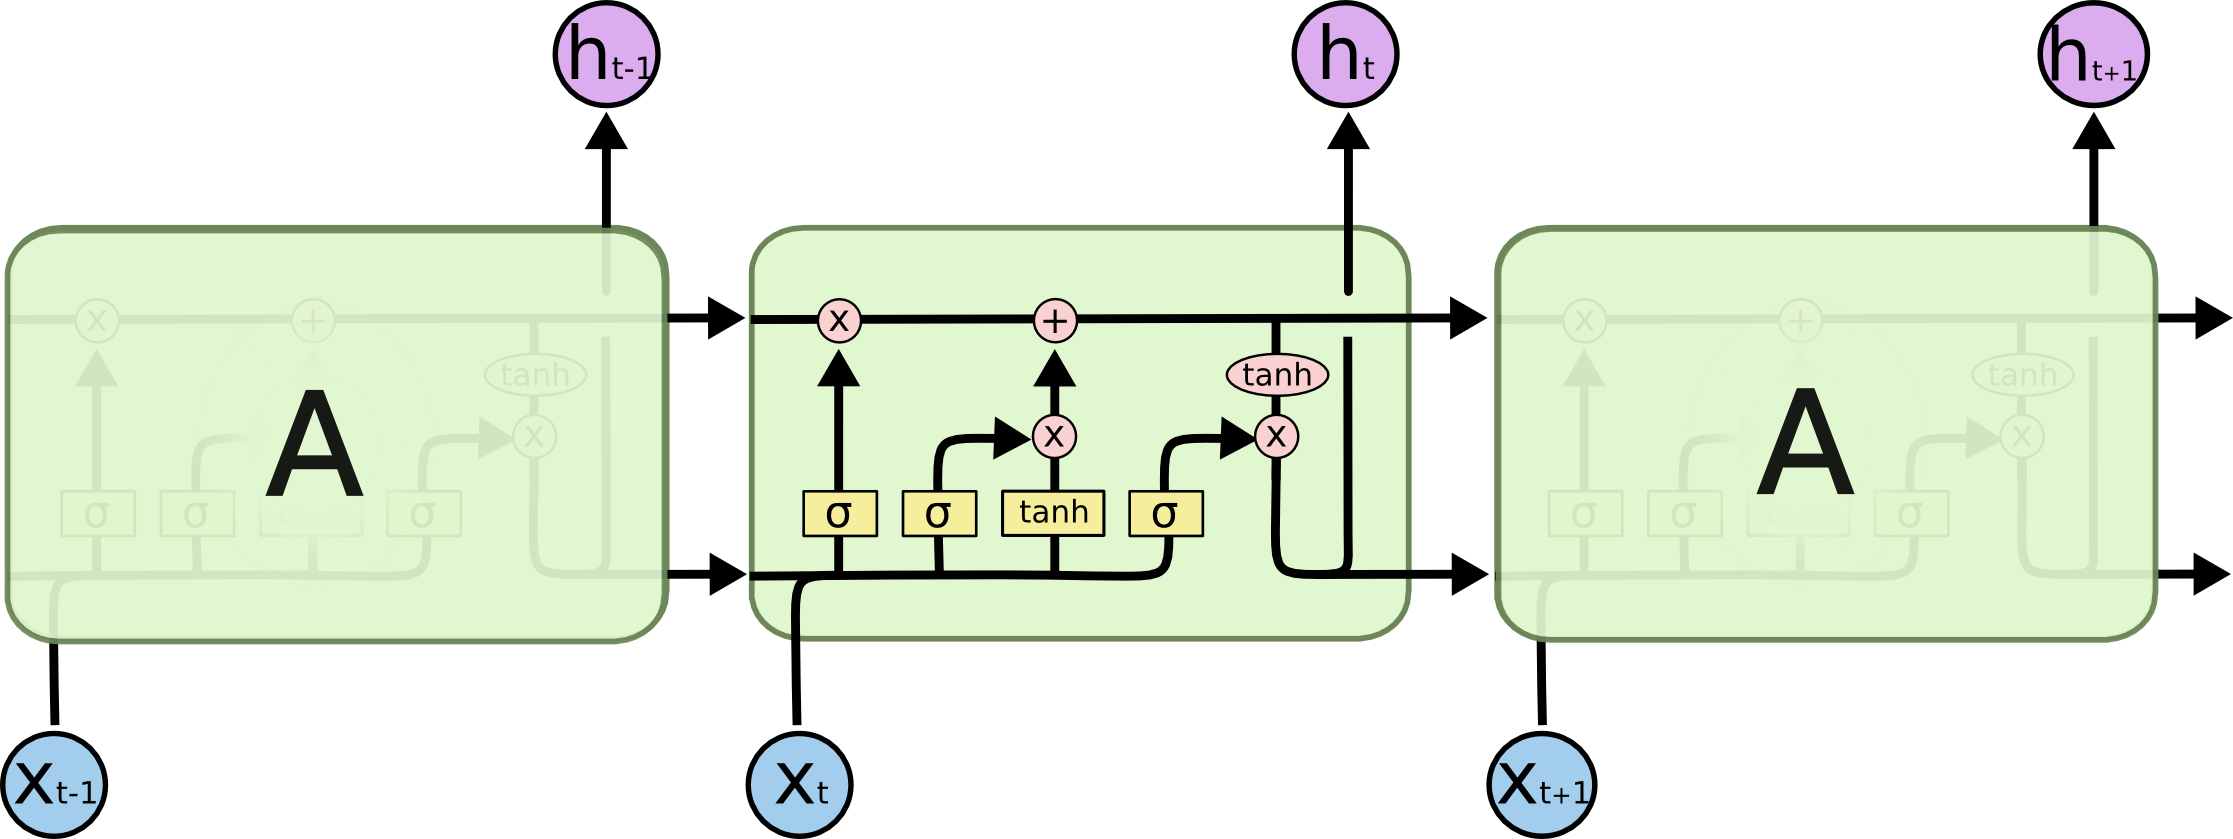
\includegraphics[width=.4\textwidth]{LSTM3-chain}    

      {\footnotesize $\triangle$ Repeating module in LSTM network {\tiny (\url{https://colah.github.io/posts/2015-08-Understanding-LSTMs/})}}
    \end{center}
    \pe
  \item A chain of LSTM cells in a network may be referred to as ``layer'' or ``block'' (usage/terminology differs)
    \pe

  \begin{center}
    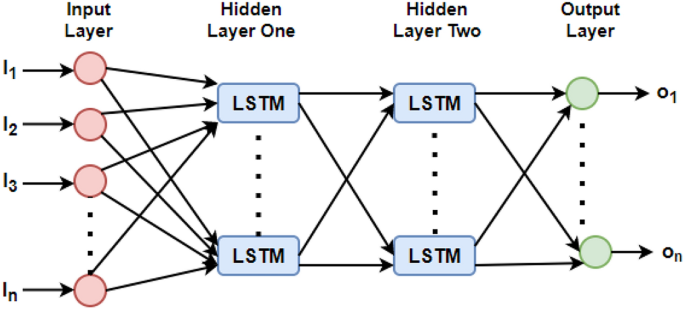
\includegraphics[width=.4\textwidth]{lstm-net}

    {\footnotesize $\triangle$ LSTM network with 2 blocks of LSTM cells
      {\tiny (\url{https://link.springer.com/article/10.1007/s42452-021-04421-x})}}
  \end{center}
\end{itemize}
% \begin{itemize}
  % \item $i$: cell (there are as many LSTM cells are there are hidden units in current implementations (e.g. Keras))\pe
  % \item $j$: input feature in $\bm x_{t}$\pe
  % \item $k$: hidden unit (element in vector $\bm h_{t}$)\pe
  % \item $t$: time step
  % \end{itemize}

\end{frame}
% \begin{frame}[fragile]
%   \frametitle{LSTM anatomy}
%   \pause

%   The LSTM cell has four neural network layers (compared to one layer in the standard RNN)


%  \begin{center}
% \begin{tikzpicture}[scale=.95,
%     % GLOBAL CFG
%     font=\sf \scriptsize,
%     >=LaTeX,
%     % Styles
%     cell/.style={% For the main box
%         rectangle, 
%         rounded corners=5mm, 
%         draw,
%         very thick,
%         },
%     operator/.style={%For operators like +  and  x
%         circle,
%         draw,
%         inner sep=-0.5pt,
%         minimum height =.2cm,
%         },
%     function/.style={%For functions
%         ellipse,
%         draw,
%         inner sep=1pt
%         },
%     ct/.style={% For external inputs and outputs
%         circle,
%         draw,
%         line width = .75pt,
%         minimum width=1cm,
%         inner sep=1pt,
%         },
%     gt/.style={% For internal inputs
%         rectangle,
%         draw,
%         minimum width=4mm,
%         minimum height=3mm,
%         inner sep=1pt
%         },
%     mylabel/.style={% something new that I have learned
%         font=\scriptsize\sffamily
%         },
%     ArrowC1/.style={% Arrows with rounded corners
%         rounded corners=.25cm,
%         thick,
%         },
%     ArrowC2/.style={% Arrows with big rounded corners
%         rounded corners=.5cm,
%         thick,
%         },
%     ]

% %Start drawing the thing...    
%     % Draw the cell: 
%     \node [cell, minimum height =4cm, minimum width=6cm] at (0,0){} ;

%     % Draw inputs named ibox#
%     \node [gt] (ibox1) at (-2,-0.75) {$\bm\sigma$};
%     \node [gt] (ibox2) at (-1.5,-0.75) {$\bm\sigma$};
%     \node [gt, minimum width=1cm] (ibox3) at (-0.5,-0.75) {tanh};
%     \node [gt] (ibox4) at (0.5,-0.75) {$\bm\sigma$};

%    % Draw opérators   named mux# , add# and func#
%     \node [operator] (mux1) at (-2,1.5) {$\times$};
%     \node [operator] (add1) at (-0.5,1.5) {+};
%     \node [operator] (mux2) at (-0.5,0) {$\times$};
%     \node [operator] (mux3) at (1.5,0) {$\times$};
%     \node [function] (func1) at (1.5,0.75) {Tanh};

%     % Draw External inputs? named as basis c,h,x
%     \node[ct, label={[mylabel]Cell State}] (c) at (-4,1.5) {\empt{c}{t-1}};
%     \node[ct, label={[mylabel]Hidden}] (h) at (-4,-1.5) {\empt{h}{t-1}};
%     \node[ct, label={[mylabel]left:Input}] (x) at (-2.5,-3) {\empt{x}{t}};

%     % Draw External outputs? named as basis c2,h2,x2
%     \node[ct, label={[mylabel]Cell State}] (c2) at (4,1.5) {\empt{c}{t}};
%     \node[ct, label={[mylabel]Hidden}] (h2) at (4,-1.5) {\empt{h}{t}};
%     \node[ct, label={[mylabel]left:Output}] (x2) at (2.5,3) {\empt{h}{t}};

% % Start connecting all.
%     %Intersections and displacements are used. 
%     % Drawing arrows    
%     \draw [ArrowC1] (c) -- (mux1) -- (add1) -- (c2);

%     % Inputs
%     \draw [ArrowC2] (h) -| (ibox4);
%     \draw [ArrowC1] (h -| ibox1)++(-0.5,0) -| (ibox1); 
%     \draw [ArrowC1] (h -| ibox2)++(-0.5,0) -| (ibox2);
%     \draw [ArrowC1] (h -| ibox3)++(-0.5,0) -| (ibox3);
%     \draw [ArrowC1] (x) -- (x |- h)-| (ibox3);

%     % Internal
%     \draw [->, ArrowC2] (ibox1) -- (mux1);
%     \draw [->, ArrowC2] (ibox2) |- (mux2);
%     \draw [->, ArrowC2] (ibox3) -- (mux2);
%     \draw [->, ArrowC2] (ibox4) |- (mux3);
%     \draw [->, ArrowC2] (mux2) -- (add1);
%     \draw [->, ArrowC1] (add1 -| func1)++(-0.5,0) -| (func1);
%     \draw [->, ArrowC2] (func1) -- (mux3);

%     %Outputs
%     \draw [-, ArrowC2] (mux3) |- (h2);
%     \draw (c2 -| x2) ++(0,-0.1) coordinate (i1);
%     \draw [-, ArrowC2] (h2 -| x2)++(-0.5,0) -| (i1);
%     \draw [-, ArrowC2] (i1)++(0,0.2) -- (x2);

%   \end{tikzpicture}
%   \end{center}
% \end{frame}

\begin{frame}
  \frametitle{LSTM gates}
  \pause

   Gates allow the LSTM to decide which signal to pass or block by outputting a number in the interval $[0,1]$ (via a sigmoid activation) \pause

   \bigskip
   
   The LSTM cell consists of three gates:
    

    \begin{itemize}
    \item \textbf{\rd Forget gate:} Decides what information will be discarded from cell state. Contained in sigmoid layer that outputs number between 0 and 1 for each number in cell state $\bm{c}_{t-1}$\pause
    \item \textbf{\og Input gate:} Decides what new information to store in cell state. Comprises
      \begin{enumerate}[\bf (a)]
      \item sigmoid layer which decides values to update \pause
      \item tanh layer to create new candidate values for the state
    \end{enumerate}
\pause
\item \textbf{\gr Output gate:} Decides what information is passed from cell state to output. Comprises
  \begin{enumerate}[\bf (a)]
  \item  sigmoid layer to decide portion of cell state to retain \pause
  \item tanh later which admits state values in $[-1,1]$
\end{enumerate}
 
    \end{itemize}

\end{frame}

\begin{frame}
  \frametitle{LSTM cell anatomy}

   \begin{center}
\begin{tikzpicture}[scale=.95,
    % GLOBAL CFG
    font=\sf \scriptsize,
    >=LaTeX,
    % Styles
    cell/.style={% For the main box
        rectangle, 
        rounded corners=5mm, 
        draw,
        very thick,
        },
    operator/.style={%For operators like +  and  x
        circle,
        draw,
        inner sep=-0.5pt,
        minimum height =.2cm,
        },
    function/.style={%For functions
        ellipse,
        draw,
        inner sep=1pt
        },
    ct/.style={% For external inputs and outputs
        circle,
        draw,
        line width = .75pt,
        minimum width=1cm,
        inner sep=1pt,
        },
    gt/.style={% For internal inputs
        rectangle,
        draw,
        minimum width=4mm,
        minimum height=3mm,
        inner sep=1pt
        },
    mylabel/.style={% something new that I have learned
        font=\scriptsize\sffamily
        },
    ArrowC1/.style={% Arrows with rounded corners
        rounded corners=.25cm,
        thick,
        },
    ArrowC2/.style={% Arrows with big rounded corners
        rounded corners=.5cm,
        thick,
        },
    ]

%Start drawing the thing...    
    % Draw the cell: 
    \node [cell, minimum height =4cm, minimum width=6cm] at (0,0){} ;

    % Draw inputs named ibox#
    \node [gt, fill=red!50!] (ibox1) at (-2,-0.75) {$\sigma$};
    \node [gt, fill=orange!50!] (ibox2) at (-1.5,-0.75) {$\sigma$};
    \node [gt, minimum width=1cm] (ibox3) at (-0.5,-0.75) {tanh};
    \node [gt, fill=green!50!] (ibox4) at (0.5,-0.75) {$\sigma$};

   % Draw opérators   named mux# , add# and func#
    \node [operator] (mux1) at (-2,1.5) {$\times$};
    \node [operator] (add1) at (-0.5,1.5) {+};
    \node [operator] (mux2) at (-0.5,0) {$\times$};
    \node [operator] (mux3) at (1.5,0) {$\times$};
    \node [function] (func1) at (1.5,0.75) {tanh};

    % Draw External inputs? named as basis c,h,x
    \node[ct, label={[mylabel]Cell State}] (c) at (-4,1.5) {\empt{c}{t-1}};
    \node[ct, label={[mylabel]Hidden}] (h) at (-4,-1.5) {\empt{h}{t-1}};
    \node[ct, label={[mylabel]left:Input}] (x) at (-2.5,-3) {\empt{x}{t}};

    % Draw External outputs? named as basis c2,h2,x2
    \node[ct, label={[mylabel]Cell State}] (c2) at (4,1.5) {\empt{c}{t}};
    \node[ct, label={[mylabel]Hidden}] (h2) at (4,-1.5) {\empt{h}{t}};
    \node[ct, label={[mylabel]left:Output}] (x2) at (2.5,3) {\empt{h}{t}};

% Start connecting all.
    %Intersections and displacements are used. 
    % Drawing arrows    
    \draw [ArrowC1] (c) -- (mux1) -- (add1) -- (c2);

    % Inputs
    \draw [ArrowC2] (h) -| (ibox4);
    \draw [ArrowC1] (h -| ibox1)++(-0.5,0) -| (ibox1); 
    \draw [ArrowC1] (h -| ibox2)++(-0.5,0) -| (ibox2);
    \draw [ArrowC1] (h -| ibox3)++(-0.5,0) -| (ibox3);
    \draw [ArrowC1] (x) -- (x |- h)-| (ibox3);

    % Internal
    \draw [->, ArrowC2] (ibox1) -- (mux1);
    \draw [->, ArrowC2] (ibox2) |- (mux2);
    \draw [->, ArrowC2] (ibox3) -- (mux2);
    \draw [->, ArrowC2] (ibox4) |- (mux3);
    \draw [->, ArrowC2] (mux2) -- (add1);
    \draw [->, ArrowC1] (add1 -| func1)++(-0.5,0) -| (func1);
    \draw [->, ArrowC2] (func1) -- (mux3);

    %Outputs
    \draw [-, ArrowC2] (mux3) |- (h2);
    \draw (c2 -| x2) ++(0,-0.1) coordinate (i1);
    \draw [-, ArrowC2] (h2 -| x2)++(-0.5,0) -| (i1);
    \draw [-, ArrowC2] (i1)++(0,0.2) -- (x2);

    % Legend:
    \node [label=right:{\rd Forget gate}, gt, fill=red!50!] (ibox1) at (2.5,-3.4) {$\sigma$} ;
    \node [label=right:{\og Input gate}, gt, fill=orange!50!] (ibox2) at (2.5,-3.8) {$\sigma$};
    \node [label=right:{\gr Output gate}, gt, fill=green!50!] (ibox4) at (2.5,-4.2) {$\sigma$} ;

  \end{tikzpicture}
\end{center}

\end{frame}



\begin{frame}
  \frametitle{Forget gate}
  \pause

  
 The forget gate determines what information should be discarded from the cell. \pe The gate unit is given by:
       \begin{equation}
    f_{t,i} = \bm\sigma\lt(b_{i}^f + \sum_{j}U_{i,j}^f x_{t,j} + \sum_{j}W_{i,k}^fh_{t-1,k}\rt)
  \end{equation}
  \pause
  where:
  \begin{itemize}
    \item $f_{t,i}$: forget gate value for timestep $t$ and cell $i$ (between 0 and 1)
  \item $\bm x_{t}$: current input vector \pause
  \item $\bm h_{t-1}$: hidden state from previous cell \pause
  \item $\bm b^{f}$, $\bm U^{f}$, $\bm W^{f}$: biases, input weights and recurrent weights for the forget gates
    \end{itemize}

\end{frame}

\begin{frame}
  \frametitle{Input gate}
  \pause

  The input gate determines what new information to include in the cell. \pe Its unit is given by:
    \pause
    \begin{equation}
      g_{t,i} = \bm\sigma\lt(b_{i}^{g} + \sum_{j}U_{i,j}^{g}x_{t,j} + \sum_{j}W_{i,k}^{g}h_{t-1,k}\rt)
    \end{equation} \pause
    where:
    \begin{itemize}
    \item $\bm b^{g}$, $\bm U^{g}$, $\bm W^{g}$: biases, input weights and recurrent weights for the input gates
    \item $\bm h_{t-1}$: hidden state from previous cell \pause
    \end{itemize}
   
\end{frame}


\begin{frame}
  \frametitle{State update}
  \pause

 
  The cell state update is given by:
     \begin{equation}
      c_{t,i} = f_{t,i}c_{t-1,i} + g_{t,i}{\pl \tanh\lt(b_{i} + \sum_{j}U_{i,j}x_{t,j} + \sum_{j}W_{i,k}h_{t-1,j}\rt)}
    \end{equation}\pause
   
    \begin{itemize}
    \item $\bm b$, $\bm U$, $\bm W$ are biases, input weights and recurrent weights, respectively, into the LSTM cell
    \item $c_{t-1,i}$ is the cell state for the prior timestep
    \item The term in {\pl purple} represents the signal from new information $\bm x_{t}$ that may be included in the cell
      state update. Let us call it $\pl \tilde{\bm c}_{t}$
 
    \item     Thus, we may write the cell state update as: \pause
    \begin{equation}
      c_{t,i} = {\rd f_{t,i}c_{t-1,i}} +{\bl g_{t,i}\tilde{c}_{t,i}}
    \end{equation}
  \item In this form, we explicitly how the cell state is composed of a weighted sum of the {\rd prior cell state (accumulated information)} and {\bl new inputs}

    
    \end{itemize}
 \end{frame}



\begin{frame}
  \frametitle{Output gate}
  \pause

     The output gate unit is given by:
    \begin{equation}
      q_{t,i} = \bm\sigma\lt(b_{i}^{o} + \sum_{j}U_{i,j}^{o}x_{t,j} + \sum_{j}W_{i,j}^{o}h_{t-1,j}\rt)
    \end{equation}
    \pause

    And the final output (hidden state) of the LSTM cell is:
    \begin{equation}
      h_{t,i} = \tanh(c_{t,i})q_{t,i}
    \end{equation}
 \end{frame}


 \begin{frame}
  \frametitle{LSTM: putting it all together}\pe

  The complete set of LSTM update equations is given by:\pe
  \begin{eqnarray}
 \bm F_t &=& \bm \sigma(\bm X_t \bm W_{xf} + \bm H_{t-1}\bm W_{hf} + \bm b_f) \\\pe
 \bm I_t &=& \bm \sigma(\bm X_t \bm W_{xi} + \bm H_{t-1}\bm W_{hi} + \bm b_i) \\\pe
  \bm O_t &=& \bm \sigma(\bm X_t \bm W_{xo} + \bm H_{t-1}\bm W_{ho} + \bm b_o) \\\pe
  \bm{\tilde{C}}_t &=& \tanh(\bm X_t \bm W_{xc} + \bm H_{t-1}\bm W_{hc} + \bm b_c) \\\pe
  \bm C_t &=& \bm F_t \odot \bm C_{t-1} + \bm I_t \odot \bm{\tilde{C}}_t \\\pe
  \bm H_t &=& \bm O_t \odot \tanh(\bm C_t)
  \end{eqnarray}
  \pe
  where:
  \begin{itemize}
  \item $\bm F_t$, $\bm I_t$, $\bm O_t$: forget, input and output gate vectors at time $t$
  \item $\bm C_t$: cell state vector at time $t$
  \item $\bm H_t$: hidden state (output) vector at time $t$
  \item $\odot$: element-wise (Hadamard) product
  \end{itemize}      
 
 \end{frame}

 \section{Attention}
 \begin{frame}
  \frametitle{Attention}\pe
  \begin{itemize}
    \item Typical neural networks process all parts of the input with equal importance: \pe
    \begin{equation}
      \bm z = \varphi (\bm W\bm v), \quad \bm v \in \mathbb{R}^v, \bm W\in\mathbb{R}^{v'\times v}  
    \end{equation}
    \pe
    \item Attention mechanisms were introduced to allow flexibility: i.e. for models to dynamically focus 
      on the most relevant portion of the input when generating each part of the output.\pe
    \item This is typically done by computing a weighted sum of the input features $\bm v_i$, where the weights are learned based on the input itself.

  \end{itemize}
\pe
\begin{center}
    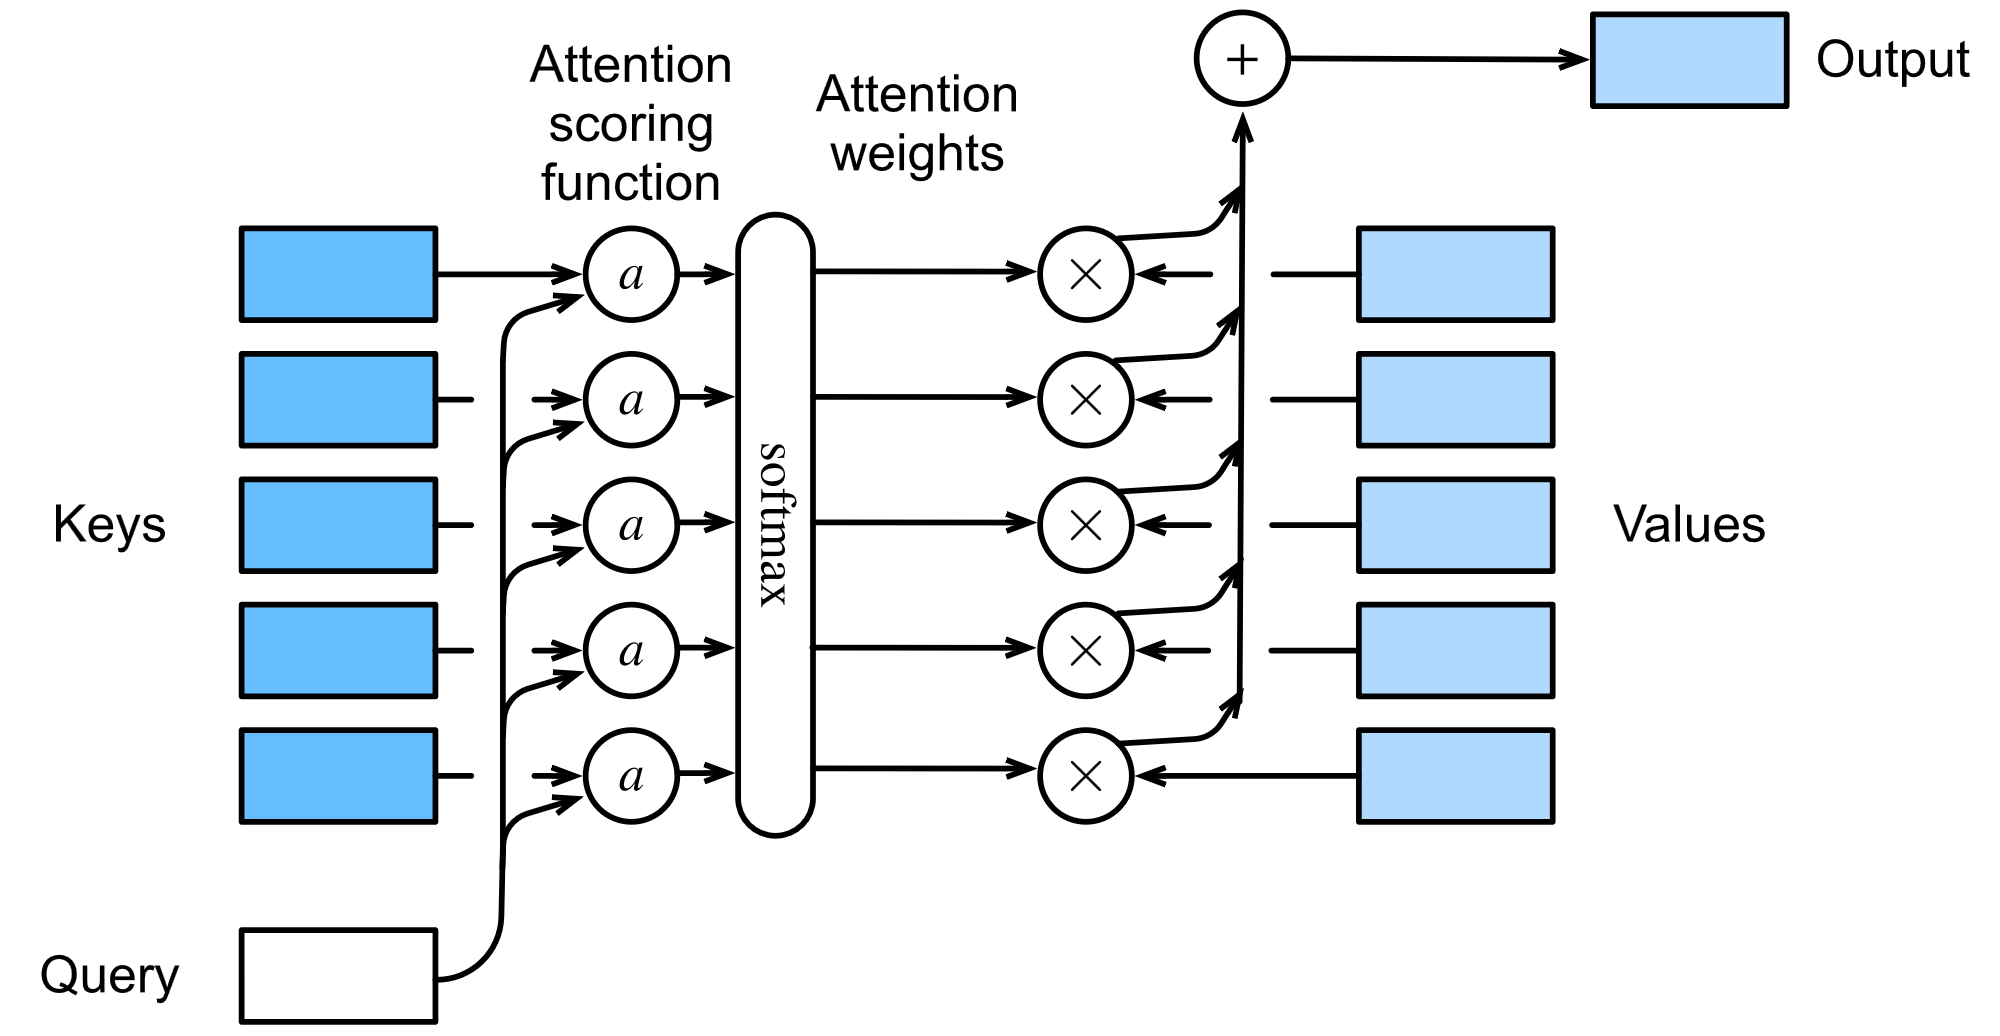
\includegraphics[width=.5\textwidth]{probml-attention.png}

    {\footnotesize $\triangle$ Attention as weighted sum of values (Source: \url{https://github.com/probml/pml-book/blob/main/book1-figures/Figure_15.16.pdf})}
\end{center}
 \end{frame}

\begin{frame}
  \frametitle{Attention scores}\pe

      \begin{itemize}
      \item Given $m$ values $\bm V \in \mathbb{R}^{m \times v}$\pe
      \item input query vector $\bm q \in \mathbb{R}^q$\pe
      \item $m$ keys $\bm K \in \mathbb{R}^{m \times k}$\pe
      \item Attention output is given by:\pe
      \begin{equation}
        \text{Attention}(\bm q, \bm K, \bm V) = \sum_{i=1}^{m} \alpha_i \bm v_i
      \end{equation}
      \pe
      where the attention weights $\alpha_i$ are computed as:\pe
      \begin{equation}
        \alpha_i = \fr{\exp( a(\bm q, \bm k_i))}{\sum_{j=1}^{m}\exp( a(\bm q, \bm k_j))} 
      \end{equation}
      \pe
      and $ a(\bm q, \bm k_i)$ is a score function that measures the similarity between the
      query $\bm q$ and key vectors $\bm k_i$.\pe
    \end{itemize}
\end{frame}

\begin{frame}
  \frametitle{Commonly used score functions}\pe
  Common choices for the score function $ a(\bm q, \bm k_i)$ include:\pe
  \begin{itemize}
  \item Dot product: \pe
    \begin{equation}
      a(\bm q, \bm k_i) = \bm q^{T}\bm k_i
    \end{equation} \pe
    Often it is scaled by $\sqrt{d}$ to ensure the variance of the score remains 1: \pe
    \begin{equation}
      a(\bm q, \bm k_i) = \fr{\bm q^{T}\bm k_i}{\sqrt{d}}
    \end{equation}
\pe
  \item Additive (Bahdanau) attention: \pe
    \begin{equation}
      a(\bm q, \bm k_i) = \bm w_{a}^{T}\tanh(\bm W_{q}\bm q + \bm W_{k}\bm k_i + \bm b_a)
    \end{equation}
    \pe
    where $\bm w_a$, $\bm W_q$, $\bm W_k$, and $\bm b_a$ are learnable parameters.
  \end{itemize} 
  

\end{frame}

\begin{frame}
  \frametitle{Transformers}\pe

  A transformer is a seq2seq model architecture that uses self-attention for the encoder and decoder in place of
  an RNN.\pe
\begin{itemize}
  \item Self-attention allows the model to weigh the importance of different words in the input sequence when encoding each word.\pe
\begin{equation}
  \bm y_i = \text{Attention}(\bm x_i, (\bm x_1, \bm x_1), \ldots, (\bm x_n, \bm x_n))
\end{equation}
\pe where query is $\bm x_i$, and keys and values are all input vectors.\pe
  \item Transformers have been shown to outperform RNNs in various NLP tasks, including machine translation and text generation.\pe
  \item Popular transformer models include BERT, GPT, and T5.
\end{itemize}
\end{frame}

\begin{frame}
  \frametitle{Self-attention for context representation}\pe

  Self-attention can allow for improved representation of context.

  \begin{center}
    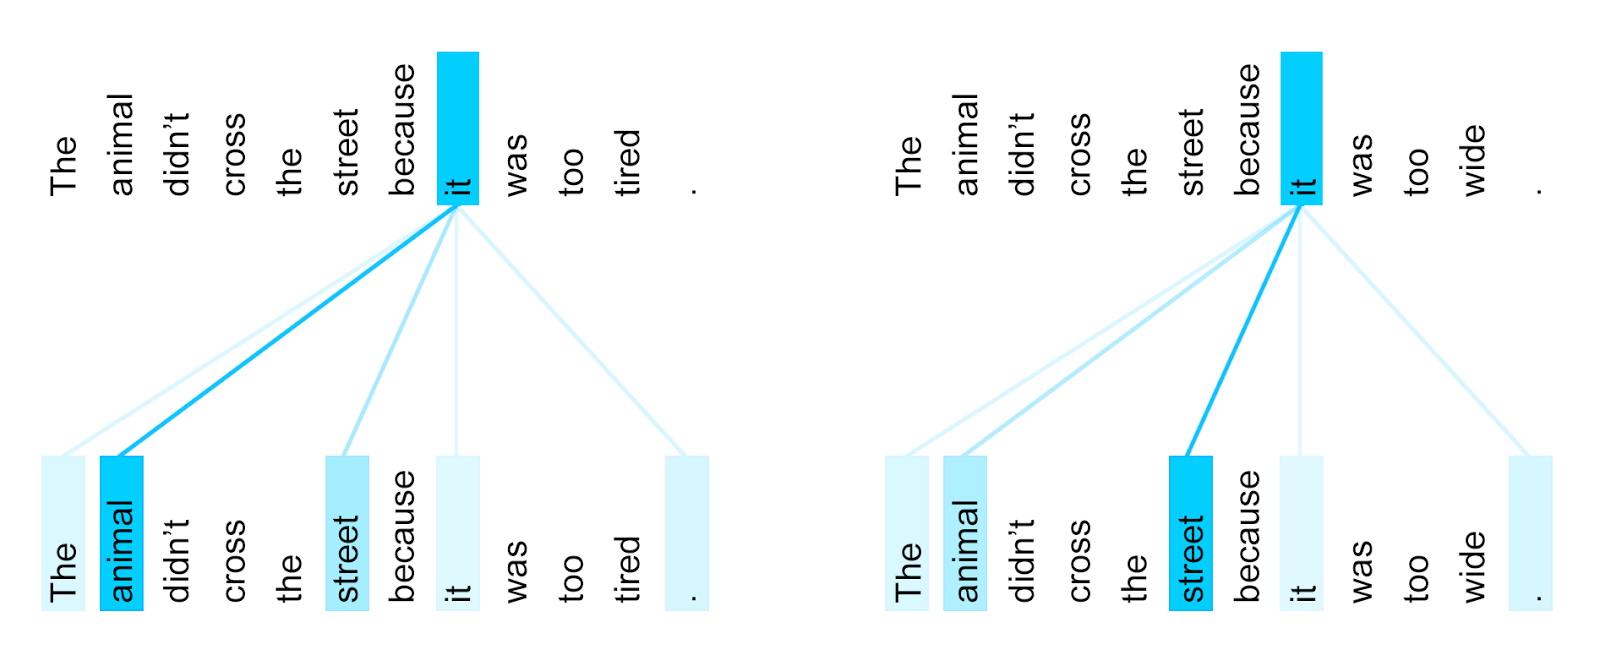
\includegraphics[width=.7\textwidth]{probml-self-attention.png}

    {\footnotesize $\triangle$ Self-attention for context representation (Source: \url{https://github.com/probml/pml-book/blob/main/book1-figures/Figure_15.23.png})}
  \end{center}

\end{frame}
 \begin{frame}
  \frametitle{Language models}\pe

  Language models are generative sequences of the form:\pe
  \begin{equation}
    p(x_1, \ldots, x_T) = \prod_{t=1}^{T}p(x_t|\bm x_{1:t-1})
  \end{equation}
  \pe
  where $x_t$ is the $t$-th word in a sequence of $T$ words.\pe

  Examples include:
 \begin{itemize}
  \item Embeddings from Language Model (ELMo)\pe
  \item Bidirectional Encoder Representations from Transformers (BERT)\pe
  \item Generative Pre-trained Transformer (GPT) models\pe
  \item Text-to-text Transfer Transformer (T5) models
 \end{itemize}
  
 
 \end{frame}
\section{Outlook}

\begin{frame}
  \frametitle{Summary}
  \begin{itemize}
  \item Recurrent neural networks are designed to learn from sequential (temporal/spatial) data
  \item The recurrence structure in RNNs renders them susceptible to the vanishing/exploding gradient problem
    \begin{itemize}
    \item It also makes it challenging for the standard RNN to learn long-term dependencies
    \end{itemize}
  \item Several approaches have been proposed to address these issues, including the use of gated RNNs
  \item LSTMs in particular are able to learn when and how much of prior information to include or forget in generating the output at each timestep
    \begin{itemize}
    \item This is done via the use of gates to control the flow of information
    \end{itemize}
  \item LSTMs have been successfully applied to handwriting recognition/generation, speech recognition, machine translation, image captioning, among others.
  \end{itemize}
\end{frame}
\begin{frame}
  \frametitle{Reading}
  \begin{itemize}
  \item Text:\textbf{PMLI} 15, DL10% (Goodfellow, et al., \textit{Deep Learning}, Ch.\ 10)
  \item Note that in DL10, the following symbology used in describing LSTMs (10.1.1.): (Commonly used counterparts that you may find in other literature are parenthesized.)
    \begin{itemize}
    \item cell state: $\bm s_{t}$ (alternative: $\bm c_{t}$)
    \item input gate: $\bm g_{t}$ (alternative: $\bm i_{t}$)
    \item output gate: $\bm q_{t}$ (alternative: $\bm o_{t}$)
    \end{itemize}
  \item I think the $f/c/i/o$ notation is easier to follow than the $f/s/g/q$ used in the DL text
    \begin{itemize}
    \item However, given that DL uses $i$ as the index for each cell, it is probably less confusing to have $i$ representing two different things.  
    \end{itemize}
  \item An excellent resource for further explanations on how LSTMs work is available on Chris Olah's blog: \url{https://colah.github.io/posts/2015-08-Understanding-LSTMs/}
  \end{itemize}
\end{frame}
\end{document}

%%% Local Variables:
%%% mode: latex
%%% TeX-master: t
%%% End:
